% Options for packages loaded elsewhere
\PassOptionsToPackage{unicode}{hyperref}
\PassOptionsToPackage{hyphens}{url}
%
\documentclass[
  ignorenonframetext,
]{beamer}
\usepackage{pgfpages}
\setbeamertemplate{caption}[numbered]
\setbeamertemplate{caption label separator}{: }
\setbeamercolor{caption name}{fg=normal text.fg}
\beamertemplatenavigationsymbolsempty
% Prevent slide breaks in the middle of a paragraph
\widowpenalties 1 10000
\raggedbottom
\setbeamertemplate{part page}{
  \centering
  \begin{beamercolorbox}[sep=16pt,center]{part title}
    \usebeamerfont{part title}\insertpart\par
  \end{beamercolorbox}
}
\setbeamertemplate{section page}{
  \centering
  \begin{beamercolorbox}[sep=12pt,center]{part title}
    \usebeamerfont{section title}\insertsection\par
  \end{beamercolorbox}
}
\setbeamertemplate{subsection page}{
  \centering
  \begin{beamercolorbox}[sep=8pt,center]{part title}
    \usebeamerfont{subsection title}\insertsubsection\par
  \end{beamercolorbox}
}
\AtBeginPart{
  \frame{\partpage}
}
\AtBeginSection{
  \ifbibliography
  \else
    \frame{\sectionpage}
  \fi
}
\AtBeginSubsection{
  \frame{\subsectionpage}
}
\usepackage{amsmath,amssymb}
\usepackage{iftex}
\ifPDFTeX
  \usepackage[T1]{fontenc}
  \usepackage[utf8]{inputenc}
  \usepackage{textcomp} % provide euro and other symbols
\else % if luatex or xetex
  \usepackage{unicode-math} % this also loads fontspec
  \defaultfontfeatures{Scale=MatchLowercase}
  \defaultfontfeatures[\rmfamily]{Ligatures=TeX,Scale=1}
\fi
\usepackage{lmodern}
\usetheme[]{Madrid}
\ifPDFTeX\else
  % xetex/luatex font selection
\fi
% Use upquote if available, for straight quotes in verbatim environments
\IfFileExists{upquote.sty}{\usepackage{upquote}}{}
\IfFileExists{microtype.sty}{% use microtype if available
  \usepackage[]{microtype}
  \UseMicrotypeSet[protrusion]{basicmath} % disable protrusion for tt fonts
}{}
\makeatletter
\@ifundefined{KOMAClassName}{% if non-KOMA class
  \IfFileExists{parskip.sty}{%
    \usepackage{parskip}
  }{% else
    \setlength{\parindent}{0pt}
    \setlength{\parskip}{6pt plus 2pt minus 1pt}}
}{% if KOMA class
  \KOMAoptions{parskip=half}}
\makeatother
\usepackage{xcolor}
\newif\ifbibliography
\usepackage{color}
\usepackage{fancyvrb}
\newcommand{\VerbBar}{|}
\newcommand{\VERB}{\Verb[commandchars=\\\{\}]}
\DefineVerbatimEnvironment{Highlighting}{Verbatim}{commandchars=\\\{\}}
% Add ',fontsize=\small' for more characters per line
\usepackage{framed}
\definecolor{shadecolor}{RGB}{248,248,248}
\newenvironment{Shaded}{\begin{snugshade}}{\end{snugshade}}
\newcommand{\AlertTok}[1]{\textcolor[rgb]{0.94,0.16,0.16}{#1}}
\newcommand{\AnnotationTok}[1]{\textcolor[rgb]{0.56,0.35,0.01}{\textbf{\textit{#1}}}}
\newcommand{\AttributeTok}[1]{\textcolor[rgb]{0.13,0.29,0.53}{#1}}
\newcommand{\BaseNTok}[1]{\textcolor[rgb]{0.00,0.00,0.81}{#1}}
\newcommand{\BuiltInTok}[1]{#1}
\newcommand{\CharTok}[1]{\textcolor[rgb]{0.31,0.60,0.02}{#1}}
\newcommand{\CommentTok}[1]{\textcolor[rgb]{0.56,0.35,0.01}{\textit{#1}}}
\newcommand{\CommentVarTok}[1]{\textcolor[rgb]{0.56,0.35,0.01}{\textbf{\textit{#1}}}}
\newcommand{\ConstantTok}[1]{\textcolor[rgb]{0.56,0.35,0.01}{#1}}
\newcommand{\ControlFlowTok}[1]{\textcolor[rgb]{0.13,0.29,0.53}{\textbf{#1}}}
\newcommand{\DataTypeTok}[1]{\textcolor[rgb]{0.13,0.29,0.53}{#1}}
\newcommand{\DecValTok}[1]{\textcolor[rgb]{0.00,0.00,0.81}{#1}}
\newcommand{\DocumentationTok}[1]{\textcolor[rgb]{0.56,0.35,0.01}{\textbf{\textit{#1}}}}
\newcommand{\ErrorTok}[1]{\textcolor[rgb]{0.64,0.00,0.00}{\textbf{#1}}}
\newcommand{\ExtensionTok}[1]{#1}
\newcommand{\FloatTok}[1]{\textcolor[rgb]{0.00,0.00,0.81}{#1}}
\newcommand{\FunctionTok}[1]{\textcolor[rgb]{0.13,0.29,0.53}{\textbf{#1}}}
\newcommand{\ImportTok}[1]{#1}
\newcommand{\InformationTok}[1]{\textcolor[rgb]{0.56,0.35,0.01}{\textbf{\textit{#1}}}}
\newcommand{\KeywordTok}[1]{\textcolor[rgb]{0.13,0.29,0.53}{\textbf{#1}}}
\newcommand{\NormalTok}[1]{#1}
\newcommand{\OperatorTok}[1]{\textcolor[rgb]{0.81,0.36,0.00}{\textbf{#1}}}
\newcommand{\OtherTok}[1]{\textcolor[rgb]{0.56,0.35,0.01}{#1}}
\newcommand{\PreprocessorTok}[1]{\textcolor[rgb]{0.56,0.35,0.01}{\textit{#1}}}
\newcommand{\RegionMarkerTok}[1]{#1}
\newcommand{\SpecialCharTok}[1]{\textcolor[rgb]{0.81,0.36,0.00}{\textbf{#1}}}
\newcommand{\SpecialStringTok}[1]{\textcolor[rgb]{0.31,0.60,0.02}{#1}}
\newcommand{\StringTok}[1]{\textcolor[rgb]{0.31,0.60,0.02}{#1}}
\newcommand{\VariableTok}[1]{\textcolor[rgb]{0.00,0.00,0.00}{#1}}
\newcommand{\VerbatimStringTok}[1]{\textcolor[rgb]{0.31,0.60,0.02}{#1}}
\newcommand{\WarningTok}[1]{\textcolor[rgb]{0.56,0.35,0.01}{\textbf{\textit{#1}}}}
\usepackage{graphicx}
\makeatletter
\def\maxwidth{\ifdim\Gin@nat@width>\linewidth\linewidth\else\Gin@nat@width\fi}
\def\maxheight{\ifdim\Gin@nat@height>\textheight\textheight\else\Gin@nat@height\fi}
\makeatother
% Scale images if necessary, so that they will not overflow the page
% margins by default, and it is still possible to overwrite the defaults
% using explicit options in \includegraphics[width, height, ...]{}
\setkeys{Gin}{width=\maxwidth,height=\maxheight,keepaspectratio}
% Set default figure placement to htbp
\makeatletter
\def\fps@figure{htbp}
\makeatother
\setlength{\emergencystretch}{3em} % prevent overfull lines
\providecommand{\tightlist}{%
  \setlength{\itemsep}{0pt}\setlength{\parskip}{0pt}}
\setcounter{secnumdepth}{-\maxdimen} % remove section numbering
\logo{
\includegraphics[height=1cm,width=3cm]{logo.png}}
\usetheme{Madrid}
\usefonttheme{serif}
\setbeamertemplate{navigation symbols}{}

\usepackage{amsmath}


\ifLuaTeX
  \usepackage{selnolig}  % disable illegal ligatures
\fi
\IfFileExists{bookmark.sty}{\usepackage{bookmark}}{\usepackage{hyperref}}
\IfFileExists{xurl.sty}{\usepackage{xurl}}{} % add URL line breaks if available
\urlstyle{same}
\hypersetup{
  pdftitle={Leksioni 1},
  pdfauthor={Endri Raco},
  hidelinks,
  pdfcreator={LaTeX via pandoc}}

\title{Leksioni 1}
\author{Endri Raco}
\date{22 April, 2024}

\begin{document}
\frame{\titlepage}

\begin{frame}[allowframebreaks]
  \tableofcontents[hideallsubsections]
\end{frame}
\hypertarget{hyrje}{%
\section*{Hyrje}\label{hyrje}}
\addcontentsline{toc}{section}{Hyrje}

\begin{frame}{Organizimi i kursit - Python}
\protect\hypertarget{organizimi-i-kursit---python}{}
\begin{itemize}
\item
  Instalimi i Python
\item
  Konceptet bazë të programimit në Python
\item
  Analizimi i të dhënave me Python
\item
  Vizualizimi i të dhënave në Python
\end{itemize}
\end{frame}

\begin{frame}{Organizimi i kursit - Python dhe GIS}
\protect\hypertarget{organizimi-i-kursit---python-dhe-gis}{}
\begin{itemize}
\item
  Procesimi i të dhënave vektor
\item
  Procesimi i të dhënave raster
\item
  Vizualizimi i të dhënave gjeografike
\item
  Lidhja me burimet gjeografike online
\end{itemize}
\end{frame}

\begin{frame}{Organizimi i kursit - Python dhe GIS}
\protect\hypertarget{organizimi-i-kursit---python-dhe-gis-1}{}
\begin{itemize}
\item
  Interpolimi hapësinor
\item
  Analiza e rrjetit hapësinor
\item
  Analiza e terrenit
\end{itemize}
\end{frame}

\hypertarget{instalimi}{%
\section*{Instalimi}\label{instalimi}}
\addcontentsline{toc}{section}{Instalimi}

\begin{frame}{Instalimi i Python-it}
\protect\hypertarget{instalimi-i-python-it}{}
\begin{itemize}
\item
  Python dhe libraritë e tij mund të instalohen lehtësisht duke përdorur
  paketa të ndryshme.
\item
  Për të instaluar Python-in, \textbf{Miniconda} është një zgjedhje e
  mirë sepse ofron një mjedis të qëndrueshëm dhe mënjanon konfliktin e
  librarive.
\end{itemize}
\end{frame}

\begin{frame}{Menaxhimi i Varësive midis librarive (dependency)}
\protect\hypertarget{menaxhimi-i-varuxebsive-midis-librarive-dependency}{}
\begin{itemize}
\item
  Python ka një numër të madh librarish të disponueshme që mund të kenë
  varësi të ndërsjella.
\item
  Është e rëndësishme që libraritë dhe versionet e tyre të punojnë mirë
  së bashku.
\item
  Menaxhimi i librarive (package managers)
\end{itemize}
\end{frame}

\begin{frame}{Pluset e përdorimit të Miniconda}
\protect\hypertarget{pluset-e-puxebrdorimit-tuxeb-miniconda}{}
\begin{itemize}
\item
  Miniconda përfshin një menaxher librarish që lehtëson instalimin dhe
  përditësimin.
\item
  Ka support shumë të mirë
\item
  Falas
\item
  Ofron ndërfaqe grafike për lehtësi përdorimi
\end{itemize}
\end{frame}

\begin{frame}{Mjediset Virtuale (Virtual environments)}
\protect\hypertarget{mjediset-virtuale-virtual-environments}{}
\begin{itemize}
\item
  Mjediset virtuale krijojnë një hapësirë të izoluar për projektet tona
  Python.
\item
  Krijimi i mjediseve virtuale ndihmon për të shmangur konfliktet midis
  librarive dhe instalimeve të ndryshme.
\item
  Mund të krijojmë mjedise të shumta dhe të kalojmë lehtësisht mes tyre.
\end{itemize}
\end{frame}

\begin{frame}{Konfigurimi dhe Dokumentimi i Mjediseve}
\protect\hypertarget{konfigurimi-dhe-dokumentimi-i-mjediseve}{}
\begin{itemize}
\item
  Përdorim skedarët \textbf{YAML} për të dokumentuar konfigurimet e
  mjediseve që krijojmë.
\item
  Në skedarët YAML, mund të përcaktojmë specifikat e mjedisit, përfshirë
  versionin e Python-it dhe libraritë që do përdorim.
\end{itemize}
\end{frame}

\begin{frame}{Konfigurimi dhe Dokumentimi i Mjediseve}
\protect\hypertarget{konfigurimi-dhe-dokumentimi-i-mjediseve-1}{}
\begin{itemize}
\tightlist
\item
  Formati tipik për mjediset Conda/Mamba është \textbf{environment.yaml}
\end{itemize}

\href{./Figs/enviroment.png}{}
\end{frame}

\begin{frame}{Praktika të Mira}
\protect\hypertarget{praktika-tuxeb-mira}{}
\begin{itemize}
\tightlist
\item
  Është një praktikë e mirë të instalojmë të gjitha libraritë (kur është
  e mundur) nga i njëjti kanal Conda, si p.sh., \textbf{conda-forge},
  dhe të mos përziejmë \textbf{Conda} dhe \textbf{Pip} për instalime
  nëse nuk është e domosdoshme.
\end{itemize}
\end{frame}

\begin{frame}{Çfarë është një Kanal Conda}
\protect\hypertarget{uxe7faruxeb-uxebshtuxeb-njuxeb-kanal-conda}{}
\begin{itemize}
\item
  Një kanal Conda është një vendndodhje/server me një adresë të dedikuar
  në internet, ku ruhen libraritë.
\item
  Kanali shërben si bazë për strehimin(repository) e librarive, dhe
  menaxherët e paketave (si Conda/Mamba) kërkojnë dhe shkarkojnë
  libraritë nga këto kanale.
\end{itemize}
\end{frame}

\begin{frame}{Instalimi i Python dhe i librarive të rekomanduara}
\protect\hypertarget{instalimi-i-python-dhe-i-librarive-tuxeb-rekomanduara}{}
\textbf{Windows:}

\begin{itemize}
\tightlist
\item
  Shkarkojmë versionin Miniconda të bazuar në Python 3 që është i
  përshtatshëm për sistemin operativ ku do punojmë.
\end{itemize}

\url{https://docs.conda.io/en/latest/miniconda.html\#latest-miniconda-installer-links}

\begin{itemize}
\tightlist
\item
  Ndjekim udhëzimet e instalimit nga faqja e Miniconda.
\end{itemize}
\end{frame}

\begin{frame}{Kontrolli i instalimit}
\protect\hypertarget{kontrolli-i-instalimit}{}
\begin{itemize}
\tightlist
\item
  Hapim \textbf{Terminalin} ose \textbf{Anaconda Prompt}
\end{itemize}

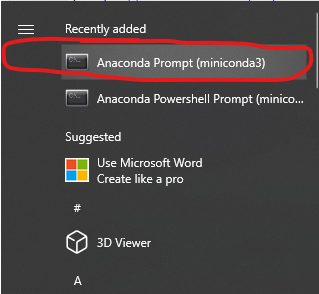
\includegraphics{./Figs/anac_prompt.png}
\end{frame}

\begin{frame}{Kontrolli i instalimit}
\protect\hypertarget{kontrolli-i-instalimit-1}{}
\begin{itemize}
\tightlist
\item
  Për të siguruar që conda është instaluar siç duhet, ekzekutojmë
  komandën:
\end{itemize}

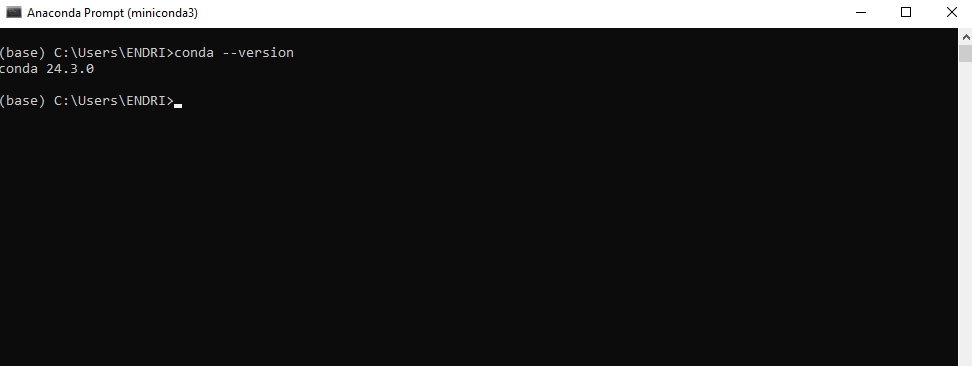
\includegraphics{./Figs/conda_ver.png}
\end{frame}

\begin{frame}[fragile]{Instalimi i Mamba}
\protect\hypertarget{instalimi-i-mamba}{}
\begin{itemize}
\item
  Mamba është një menaxher librarish për Miniconda.
\item
  Për të instaluar \textbf{mamba}, hapim \textbf{Terminalin} ose
  \textbf{Command Prompt} në Windows si administrator.
\item
  Ekzekutojmë komandën:
\end{itemize}

\begin{Shaded}
\begin{Highlighting}[]
\NormalTok{  conda install mamba {-}n base {-}c conda{-}forge}
\end{Highlighting}
\end{Shaded}
\end{frame}

\begin{frame}{Shkarkimi i Skedarit të Mjedisit Python}
\protect\hypertarget{shkarkimi-i-skedarit-tuxeb-mjedisit-python}{}
\begin{itemize}
\item
  Do përdorim skedarin \textbf{environment.yml} që përmban listën e
  librarive të nevojshme
\item
  Hapim Terminalin dhe shkoni te direktoria ku keni shkarkuar
  \href{https://github.com/endri81/instatgis/blob/master/environment.yml}{environment.yml}
\end{itemize}
\end{frame}

\begin{frame}[fragile]{Mjedisi Python}
\protect\hypertarget{mjedisi-python}{}
\begin{itemize}
\tightlist
\item
  Krijojmë mjedisin Python duke ekzekutuar:
\end{itemize}

\begin{Shaded}
\begin{Highlighting}[]
\NormalTok{mamba env create {-}f environment.yml}
\end{Highlighting}
\end{Shaded}
\end{frame}

\begin{frame}[fragile]{Mjedisi Python}
\protect\hypertarget{mjedisi-python-1}{}
Për të aktivizuar mjedisin e ri:

\begin{Shaded}
\begin{Highlighting}[]
\NormalTok{conda activate pythongis}
\end{Highlighting}
\end{Shaded}
\end{frame}

\begin{frame}[fragile]{Ekzekutimi i JupyterLab}
\protect\hypertarget{ekzekutimi-i-jupyterlab}{}
\begin{itemize}
\tightlist
\item
  Për të filluar \textbf{JupyterLab}, ekzekutojmë komandën në
  \textbf{Terminal} ose \textbf{Command Prompt}:
\end{itemize}

\begin{Shaded}
\begin{Highlighting}[]
\NormalTok{jupyter lab}
\end{Highlighting}
\end{Shaded}
\end{frame}

\begin{frame}{Ekzekutimi i JupyterLab}
\protect\hypertarget{ekzekutimi-i-jupyterlab-1}{}
\begin{itemize}
\tightlist
\item
  JupyterLab duhet të hapet automatikisht në një faqe browser
\end{itemize}
\end{frame}

\begin{frame}[fragile]{Instalimi i Librarive Shtesë}
\protect\hypertarget{instalimi-i-librarive-shtesuxeb}{}
Për të instaluar paketa të reja, përdorim komandën:

\begin{Shaded}
\begin{Highlighting}[]
\NormalTok{mamba install {-}c conda{-}forge package{-}name}
\end{Highlighting}
\end{Shaded}
\end{frame}

\begin{frame}[fragile]{Instalimi i Librarive Shtesë}
\protect\hypertarget{instalimi-i-librarive-shtesuxeb-1}{}
\begin{itemize}
\tightlist
\item
  Një shembull për instalimin e librarisë pandas nga kanali conda-forge:
\end{itemize}

\begin{Shaded}
\begin{Highlighting}[]
\NormalTok{mamba install {-}c conda{-}forge pandas}
\end{Highlighting}
\end{Shaded}
\end{frame}

\begin{frame}[fragile]{Instalimi i Librarive Shtesë}
\protect\hypertarget{instalimi-i-librarive-shtesuxeb-2}{}
\begin{itemize}
\tightlist
\item
  Në rast se shfaqet ndonjë gabim, kontrollojmë versionet dhe kanalet e
  librarive ekzistuese me komandën:
\end{itemize}

\begin{Shaded}
\begin{Highlighting}[]
\NormalTok{mamba list}
\end{Highlighting}
\end{Shaded}
\end{frame}

\begin{frame}{Çfarë është JupyterLab?}
\protect\hypertarget{uxe7faruxeb-uxebshtuxeb-jupyterlab}{}
\begin{itemize}
\item
  JupyterLab është një mjet programimi i bazuar në shfletues (browser)
  për programim dhe data science.
\item
  Ofron një mjedis të integruar që përfshin interpretues Python,
  redaktor teksti, terminal, dhe shumë më tepër.
\end{itemize}
\end{frame}

\begin{frame}{Përbërësit Kryesorë të JupyterLab}
\protect\hypertarget{puxebrbuxebruxebsit-kryesoruxeb-tuxeb-jupyterlab}{}
\begin{itemize}
\tightlist
\item
  \textbf{File Browser (Paneli i Navigimit)}:
\end{itemize}

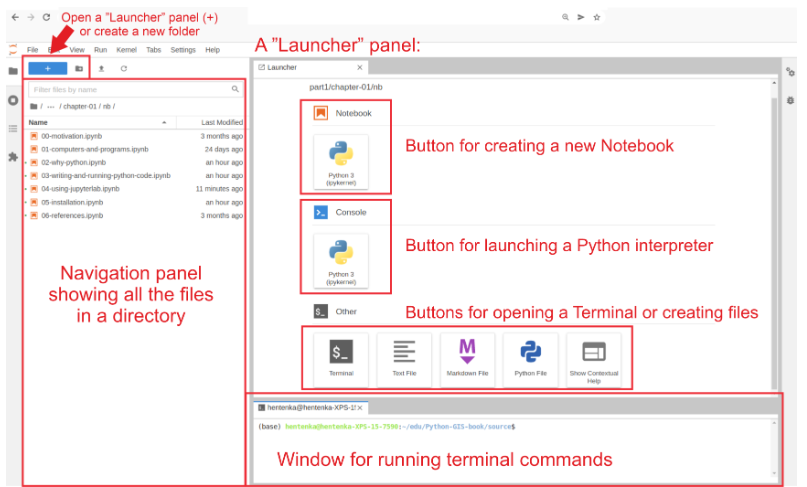
\includegraphics{./Figs/jupyter1.png} \#\# Përbërësit Kryesorë të
JupyterLab

\begin{itemize}
\item
  I vendosur në anën e majtë të ndërfaqes.
\item
  Përdoret për të naviguar në sistemin e skedarëve, për të krijuar
  skedarë të rinj ose dosje (folder).
\item
  Mund të hapim një skedar duke double-klikuar mbi të.
\item
  Për opsione të tjera, siç janë riemërtimi, kopjimi, ose fshirja e
  skedarëve, klikojmë me butonin e djathtë.
\end{itemize}
\end{frame}

\begin{frame}{Përbërësit Kryesorë të JupyterLab}
\protect\hypertarget{puxebrbuxebruxebsit-kryesoruxeb-tuxeb-jupyterlab-1}{}
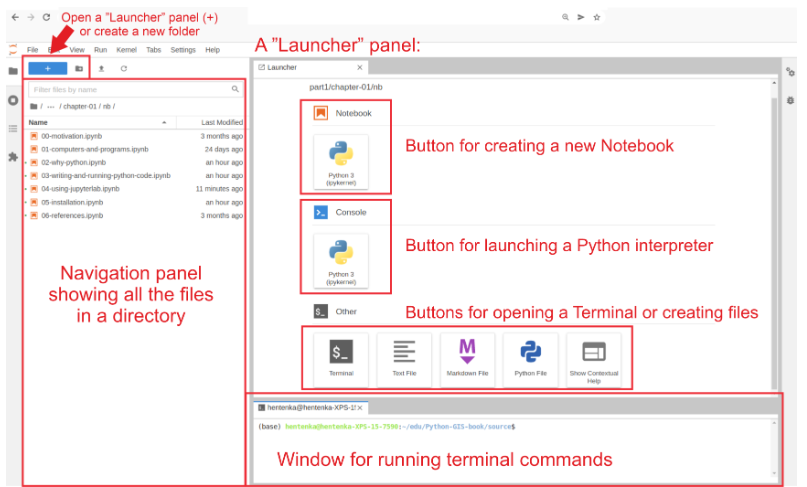
\includegraphics{./Figs/jupyter1.png}
\end{frame}

\begin{frame}{Përbërësit Kryesorë të JupyterLab}
\protect\hypertarget{puxebrbuxebruxebsit-kryesoruxeb-tuxeb-jupyterlab-2}{}
\begin{itemize}
\item
  \textbf{Launcher Panel (Paneli i Nisjes)}:

  \begin{itemize}
  \item
    I vendosur në të djathtë të ndërfaqes.
  \item
    Përdoret për të krijuar elemente të rinj, si Jupyter Notebooks,
    skedarë të rinj teksti, ose terminale të reja.
  \item
    Mund të krijojmë dokumente të reja ose sesione të reja për programim
    nga ky panel.
  \end{itemize}
\end{itemize}
\end{frame}

\begin{frame}{Përbërësit Kryesorë të JupyterLab}
\protect\hypertarget{puxebrbuxebruxebsit-kryesoruxeb-tuxeb-jupyterlab-3}{}
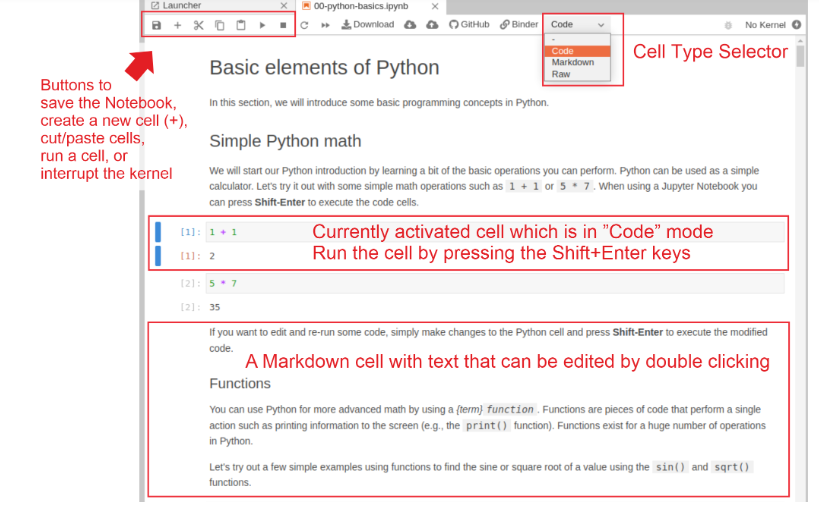
\includegraphics{./Figs/jupyter2.png}
\end{frame}

\hypertarget{programimi-bazik-nuxeb-python}{%
\section*{Programimi bazik në
Python}\label{programimi-bazik-nuxeb-python}}
\addcontentsline{toc}{section}{Programimi bazik në Python}

\hypertarget{matematika-e-thjeshtuxeb-nuxeb-python}{%
\section*{Matematika e Thjeshtë në
Python}\label{matematika-e-thjeshtuxeb-nuxeb-python}}
\addcontentsline{toc}{section}{Matematika e Thjeshtë në Python}

\begin{frame}[fragile]{Veprimet Bazë Matematike}
\protect\hypertarget{veprimet-bazuxeb-matematike}{}
\begin{itemize}
\item
  Python mund të përdoret për të kryer operacione të thjeshta
  matematikore.
\item
  Shembuj: \texttt{1\ +\ 1}, \texttt{5\ *\ 7}, \texttt{10\ /\ 2},
  \texttt{2\ **\ 3}.
\end{itemize}
\end{frame}

\begin{frame}{Veprimet Bazë Matematike}
\protect\hypertarget{veprimet-bazuxeb-matematike-1}{}
\begin{itemize}
\tightlist
\item
  Në Jupyter Notebook, shtypim \textbf{Shift-Enter} për të ekzekutuar
  kodin.
\end{itemize}

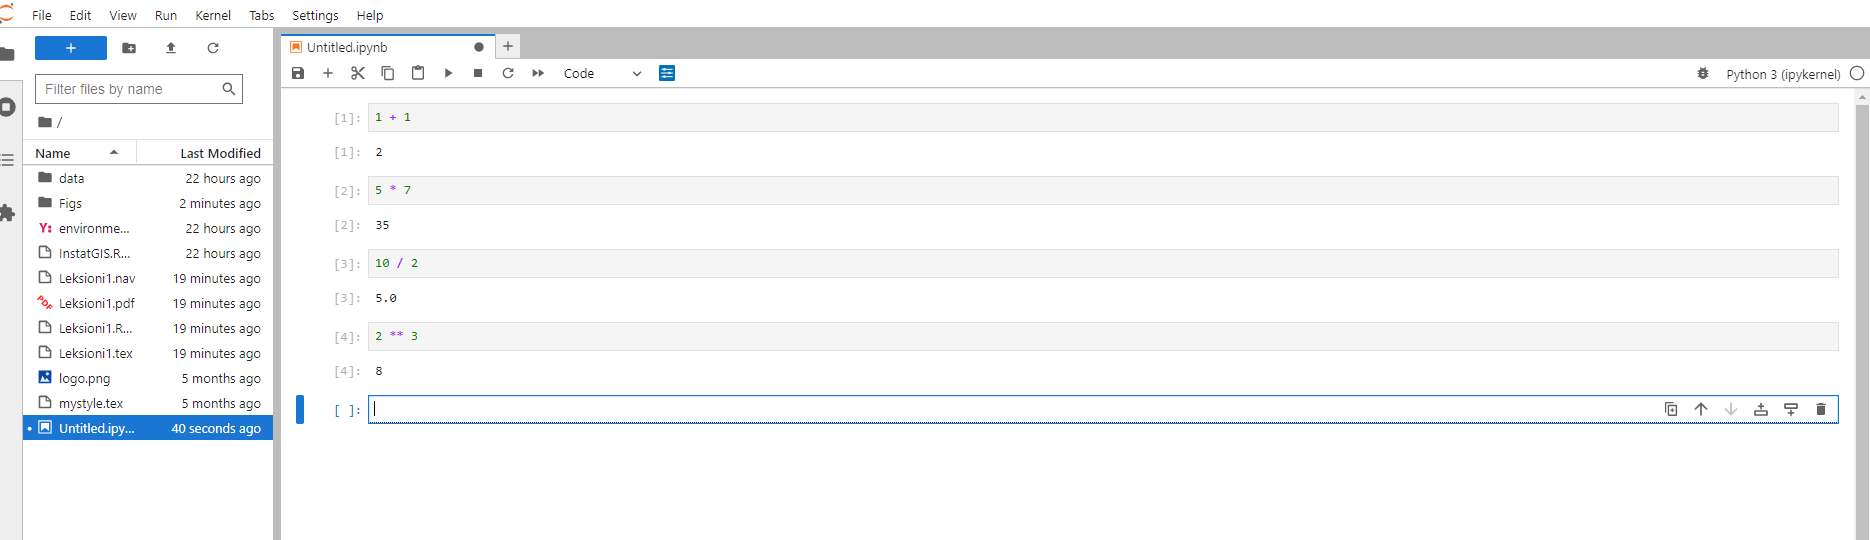
\includegraphics{./Figs/math1.png}
\end{frame}

\begin{frame}{Më shumë Veprime}
\protect\hypertarget{muxeb-shumuxeb-veprime}{}
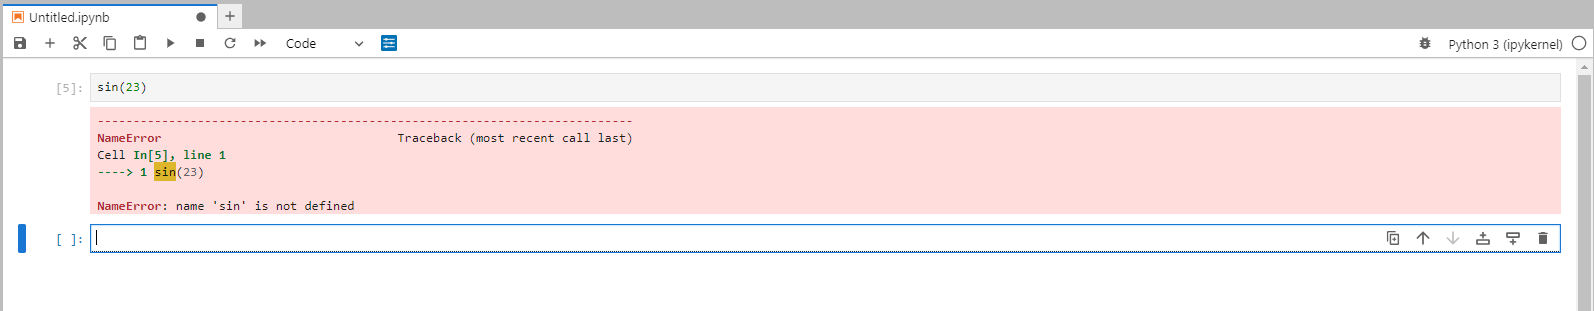
\includegraphics{./Figs/math2.png}
\end{frame}

\begin{frame}{Çfarë është Një Funksion?}
\protect\hypertarget{uxe7faruxeb-uxebshtuxeb-njuxeb-funksion}{}
\begin{itemize}
\item
  Funksionet janë pjesë të kodit që kryejnë një veprim të vetëm, si
  p.sh., printimi i informacionit në ekran.
\item
  Python ka një shumëllojshmëri të madhe funksionesh për operacione të
  ndryshme.
\end{itemize}
\end{frame}

\begin{frame}{Shembuj të Funksioneve Bazë}
\protect\hypertarget{shembuj-tuxeb-funksioneve-bazuxeb}{}
\begin{itemize}
\item
  Funksioni \textbf{print()} përdoret për të shfaqur tekst në ekran.
\item
  Funksioni \textbf{len()} kthen gjatësinë e një liste ose vargu.
\item
  Funksioni \textbf{sum()} llogarit shumën e elementeve në një listë.
\end{itemize}
\end{frame}

\begin{frame}[fragile]{Më shumë Veprime}
\protect\hypertarget{muxeb-shumuxeb-veprime-1}{}
\begin{itemize}
\item
  Për të bërë veprime më komplekse, përdorim module të tilla si
  \texttt{math}.
\item
  Importojmë modulin \texttt{math} për të përdorur funksione si
  \texttt{math.sin()}, \texttt{math.sqrt()}, etj.
\end{itemize}
\end{frame}

\begin{frame}[fragile]{Shembull}
\protect\hypertarget{shembull}{}
\begin{Shaded}
\begin{Highlighting}[]
  \ImportTok{import}\NormalTok{ math}
\NormalTok{  math.sin(}\DecValTok{3}\NormalTok{)}
\NormalTok{  math.sqrt(}\DecValTok{4}\NormalTok{)}
\end{Highlighting}
\end{Shaded}
\end{frame}

\begin{frame}{Shembull}
\protect\hypertarget{shembull-1}{}
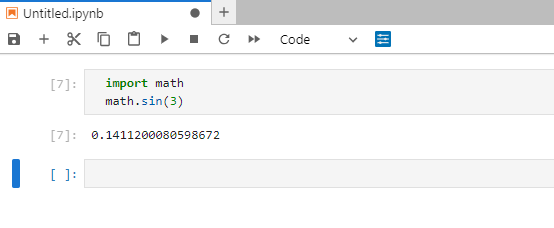
\includegraphics{./Figs/math3.png}
\end{frame}

\begin{frame}{Përmbledhje}
\protect\hypertarget{puxebrmbledhje}{}
Ja përmbledhja e asaj që pamë:

\begin{itemize}
\item
  Çfarë Është Një Modul?

  \begin{itemize}
  \item
    Një modul është një grup pjesësh kodi, si p.sh funksione, që janë të
    lidhura me njëri-tjetrin.
  \item
    Modulet individuale shpesh përfshihen në një grup të quajtur
    bibliotekë.
  \end{itemize}
\end{itemize}
\end{frame}

\begin{frame}{Përmbledhje}
\protect\hypertarget{puxebrmbledhje-1}{}
\begin{itemize}
\item
  Si Të Ngarkoni Një Modul?

  \begin{itemize}
  \item
    Për të ngarkuar një modul, përdorni deklaratën \textbf{import}.
  \item
    Funksionet që janë pjesë e një moduli mund të përdoren duke shkruar
    \textbf{modulename.functionname()}
  \item
    Për shembull, \textbf{sin()} është një funksion i modulit
    \textbf{math}, dhe përdoret duke shkruar \textbf{math.sin()} me një
    numër brenda kllapave.
  \end{itemize}
\end{itemize}
\end{frame}

\begin{frame}{Përmbledhje}
\protect\hypertarget{puxebrmbledhje-2}{}
\begin{itemize}
\item
  Përdorimi i Moduleve në Jupyter Notebook

  \begin{itemize}
  \item
    Në Jupyter Notebook, variablat që përcaktohen në qelizat e mëparshme
    janë të disponueshme për përdorim në qelizat që pasojnë, për sa kohë
    që ato janë ekzekutuar më parë.
  \item
    Kjo lejon ruajtjen e variablave për përdorim të mëtejshëm gjatë
    ekzekutimit të kodit. Konstantet në Module
  \item
    Modulet gjithashtu mund të përmbajnë konstante si \textbf{math.pi}
  \end{itemize}
\end{itemize}

\emph{Për të thirrur konstante, nuk përdoren kllapa; thjesht shkruajmë
emrin e konstantes}
\end{frame}

\hypertarget{kombinimi-i-funksioneve-nuxeb-python}{%
\section*{Kombinimi i Funksioneve në
Python}\label{kombinimi-i-funksioneve-nuxeb-python}}
\addcontentsline{toc}{section}{Kombinimi i Funksioneve në Python}

\begin{frame}[fragile]{Kombinimi i Funksioneve me print()}
\protect\hypertarget{kombinimi-i-funksioneve-me-print}{}
\begin{itemize}
\item
  Funksioni \texttt{print()} shfaq tekstin në ekran.
\item
  Për të printuar rezultatin e një funksioni tjetër, përdorim
  \texttt{print()} brenda kodit:
\end{itemize}

\begin{Shaded}
\begin{Highlighting}[]
  \ImportTok{import}\NormalTok{ math}
  \BuiltInTok{print}\NormalTok{(math.sqrt(}\DecValTok{4}\NormalTok{))  }\CommentTok{\# Shfaq 2.0}
\end{Highlighting}
\end{Shaded}
\end{frame}

\begin{frame}[fragile]{Kombinimi i Tekstit me Vlerat e Llogaritura}
\protect\hypertarget{kombinimi-i-tekstit-me-vlerat-e-llogaritura}{}
\begin{itemize}
\tightlist
\item
  Përdorim \textbf{print()} për të shfaqur tekst dhe vlera të
  llogaritura së bashku.
\end{itemize}

Shembull:

\begin{Shaded}
\begin{Highlighting}[]
\BuiltInTok{print}\NormalTok{(}\StringTok{"Dy plus dy është"}\NormalTok{, }\DecValTok{2} \OperatorTok{+} \DecValTok{2}\NormalTok{)  }\CommentTok{\# Shfaq "Dy plus dy është 4"}
\end{Highlighting}
\end{Shaded}
\end{frame}

\begin{frame}[fragile]{Kombinimi i Funksioneve}
\protect\hypertarget{kombinimi-i-funksioneve}{}
\begin{itemize}
\tightlist
\item
  Kombinojmë funksione të ndryshme për të prodhuar rezultat më të
  avancuar:
\end{itemize}

Shembull:

\begin{Shaded}
\begin{Highlighting}[]
\BuiltInTok{print}\NormalTok{(}\StringTok{"Rrënja katrore e 4 është"}\NormalTok{, math.sqrt(}\DecValTok{4}\NormalTok{))}
\end{Highlighting}
\end{Shaded}
\end{frame}

\begin{frame}[fragile]{Përdorimi i Variablave në Python}
\protect\hypertarget{puxebrdorimi-i-variablave-nuxeb-python}{}
\begin{itemize}
\tightlist
\item
  Për të caktuar vlerën e një variabli, përdorni \texttt{=}:
\end{itemize}

\begin{Shaded}
\begin{Highlighting}[]
\NormalTok{  temp\_celsius }\OperatorTok{=} \FloatTok{10.0}
\end{Highlighting}
\end{Shaded}
\end{frame}

\begin{frame}[fragile]{Përdorimi i Variablave në Python}
\protect\hypertarget{puxebrdorimi-i-variablave-nuxeb-python-1}{}
\begin{itemize}
\tightlist
\item
  Për të parë vlerën e një variabli, përdorim \textbf{print()} ose
  thjesht emrin e variablit në një qelizë Jupyter Notebook:
\end{itemize}

\begin{Shaded}
\begin{Highlighting}[]
\NormalTok{temp\_celsius  }\CommentTok{\# Kthen 10.0}
\end{Highlighting}
\end{Shaded}
\end{frame}

\begin{frame}[fragile]{Kombinimi i Variablave me Tekst}
\protect\hypertarget{kombinimi-i-variablave-me-tekst}{}
\begin{itemize}
\tightlist
\item
  Për të kombinuar tekst dhe vlera të llogaritura, përdorim
  \textbf{print()}
\end{itemize}

Shembull:

\begin{Shaded}
\begin{Highlighting}[]
\BuiltInTok{print}\NormalTok{(}\StringTok{"Temperatura në Fahrenheit:"}\NormalTok{, }\DecValTok{9} \OperatorTok{/} \DecValTok{5} \OperatorTok{*}\NormalTok{ temp\_celsius }\OperatorTok{+} \DecValTok{32}\NormalTok{)  }\CommentTok{\# Shfaq "Temperatura në Fahrenheit: 50.0"}
\end{Highlighting}
\end{Shaded}
\end{frame}

\begin{frame}[fragile]{Përditësimi i Variablave}
\protect\hypertarget{puxebrdituxebsimi-i-variablave}{}
\begin{itemize}
\tightlist
\item
  Variablat mund të përditësohen me vlera të reja:
\end{itemize}

Shembull:

\begin{Shaded}
\begin{Highlighting}[]
\NormalTok{temp\_celsius }\OperatorTok{=} \FloatTok{15.0}
\BuiltInTok{print}\NormalTok{(}\StringTok{"Temperatura në Celsius është tani:"}\NormalTok{, temp\_celsius)}
\end{Highlighting}
\end{Shaded}
\end{frame}

\begin{frame}{Kujdes me Gabimet}
\protect\hypertarget{kujdes-me-gabimet}{}
\begin{itemize}
\tightlist
\item
  Nëse përpiqeni të përdorni një variabël që nuk është definuar, do të
  merrni një \textbf{NameError}
\end{itemize}
\end{frame}

\begin{frame}[fragile]{Trajtimi i Gabimeve të Zakonshme në Python}
\protect\hypertarget{trajtimi-i-gabimeve-tuxeb-zakonshme-nuxeb-python}{}
Gabimi \textbf{NameError}

\begin{itemize}
\tightlist
\item
  Ky gabim ndodh kur një variabël ose funksion nuk është definuar.
\end{itemize}

\begin{Shaded}
\begin{Highlighting}[]
\BuiltInTok{print}\NormalTok{(}\StringTok{"Temperature in Celsius:"}\NormalTok{, }\DecValTok{5} \OperatorTok{/} \DecValTok{9} \OperatorTok{*}\NormalTok{ (tempFahrenheit }\OperatorTok{{-}} \DecValTok{32}\NormalTok{))}
\end{Highlighting}
\end{Shaded}
\end{frame}

\begin{frame}[fragile]{Trajtimi i Gabimeve të Zakonshme në Python}
\protect\hypertarget{trajtimi-i-gabimeve-tuxeb-zakonshme-nuxeb-python-1}{}
\begin{itemize}
\tightlist
\item
  Për të zgjidhur këtë gabim, sigurohemi që të gjitha variablat dhe
  funksionet të jenë të definuara dhe të importuara siç duhet.
\end{itemize}

\begin{Shaded}
\begin{Highlighting}[]
\NormalTok{tempFahrenheit }\OperatorTok{=} \DecValTok{9} \OperatorTok{/} \DecValTok{5} \OperatorTok{*}\NormalTok{ temp\_celsius }\OperatorTok{+} \DecValTok{32}
\end{Highlighting}
\end{Shaded}
\end{frame}

\hypertarget{llojet-e-tuxeb-dhuxebnave-nuxeb-python}{%
\section*{Llojet e të Dhënave në
Python}\label{llojet-e-tuxeb-dhuxebnave-nuxeb-python}}
\addcontentsline{toc}{section}{Llojet e të Dhënave në Python}

\begin{frame}{Llojet e të Dhënave në Python}
\protect\hypertarget{llojet-e-tuxeb-dhuxebnave-nuxeb-python-1}{}
\begin{itemize}
\item
  Lloji i të dhënave përcakton karakteristikat e të dhënave në një
  program.
\item
  Python ka katër lloje bazë të të dhënave: \emph{int, float, str} dhe
  \emph{bool}.
\end{itemize}
\end{frame}

\begin{frame}{Llojet Bazë të të Dhënave}
\protect\hypertarget{llojet-bazuxeb-tuxeb-tuxeb-dhuxebnave}{}
\begin{itemize}
\item
  \textbf{int:} vlera të plota të numrave të plotë.
\item
  \textbf{float:} vlera dhjetore.
\item
  \textbf{str:} vargje karakteresh (tekste).
\item
  \textbf{bool:} vlera të tipit të vërtetë/false.
\end{itemize}
\end{frame}

\begin{frame}{Shembuj të Llojeve të të Dhënave}
\protect\hypertarget{shembuj-tuxeb-llojeve-tuxeb-tuxeb-dhuxebnave}{}
int: 4

float: 3.1415

str: `Hot'

bool: True
\end{frame}

\begin{frame}[fragile]{Kontrollimi i Llojit të të Dhënave}
\protect\hypertarget{kontrollimi-i-llojit-tuxeb-tuxeb-dhuxebnave}{}
\begin{itemize}
\tightlist
\item
  Përdorim funksionin \textbf{type()} për të marrë llojin e të dhënave
  të një variabli.
\end{itemize}

Shembull:

\begin{Shaded}
\begin{Highlighting}[]
\NormalTok{weatherForecast }\OperatorTok{=} \StringTok{"Hot"}
\BuiltInTok{type}\NormalTok{(weatherForecast)  }\CommentTok{\# Kthen "str"}
\end{Highlighting}
\end{Shaded}
\end{frame}

\begin{frame}{Kujdes me Llojet e Dhënave}
\protect\hypertarget{kujdes-me-llojet-e-dhuxebnave}{}
\begin{itemize}
\item
  Llojet e të dhënave janë të rëndësishme sepse disa prej tyre nuk janë
  kompatibël me njëri-tjetrin.
\item
  Për shembull, nuk mund të mbledhim një int me një str.
\end{itemize}
\end{frame}

\begin{frame}[fragile]{Trajtimi i Gabimeve të Zakonshme në Python}
\protect\hypertarget{trajtimi-i-gabimeve-tuxeb-zakonshme-nuxeb-python-2}{}
Gabimi \textbf{TypeError}

\begin{itemize}
\tightlist
\item
  Ky gabim ndodh kur përpiqeni të kryejmë operacione me tipe të ndryshme
  të dhënave që nuk janë kompatibël.
\end{itemize}

Shembull:

\begin{Shaded}
\begin{Highlighting}[]
\NormalTok{  tempFahrenheit }\OperatorTok{+} \FloatTok{5.0} \OperatorTok{*} \StringTok{"Hot"}  \CommentTok{\# Kthen TypeError}
\end{Highlighting}
\end{Shaded}

\begin{itemize}
\tightlist
\item
  Për të shmangur këtë gabim, sigurohemi që të gjitha llojet e dhënave
  të jenë të kompatibël përpara se të kryejmë veprime.
\end{itemize}
\end{frame}

\begin{frame}{Çfarë Është Një Listë?}
\protect\hypertarget{uxe7faruxeb-uxebshtuxeb-njuxeb-listuxeb}{}
\begin{itemize}
\item
  Një listë është një koleksion vlerash të lidhura së bashku me një
  variabël të vetme.
\item
  Listat mund të përmbajnë lloje të ndryshme të dhënash, si numra,
  vargje, ose madje edhe lista të tjera.
\end{itemize}
\end{frame}

\begin{frame}[fragile]{Krijimi i Një Liste}
\protect\hypertarget{krijimi-i-njuxeb-liste}{}
\begin{itemize}
\item
  Për të krijuar një listë, përdorim kllapat katrore \texttt{{[}{]}} dhe
  ndajmë elementët me presje.
\item
  Shembull:
\end{itemize}

\begin{Shaded}
\begin{Highlighting}[]
\NormalTok{  station\_names }\OperatorTok{=}\NormalTok{ [}\StringTok{"Tirane"}\NormalTok{, }\StringTok{"Durrës"}\NormalTok{, }\StringTok{"Elbasan"}\NormalTok{, }\StringTok{"Sarandë"}\NormalTok{]  }
\end{Highlighting}
\end{Shaded}
\end{frame}

\begin{frame}[fragile]{Kontrollimi i Llojit të Një Liste}
\protect\hypertarget{kontrollimi-i-llojit-tuxeb-njuxeb-liste}{}
\begin{itemize}
\item
  Përdorim funksionin \textbf{type()} për të kontrolluar nëse një
  variabël është një listë.
\item
  Shembull:
\end{itemize}

\begin{Shaded}
\begin{Highlighting}[]
\BuiltInTok{type}\NormalTok{(station\_names)  }\CommentTok{\# Kthen "list"}
\end{Highlighting}
\end{Shaded}
\end{frame}

\begin{frame}{Përdorimi i Listave}
\protect\hypertarget{puxebrdorimi-i-listave}{}
\begin{itemize}
\item
  Listat mund të përdoren për të ruajtur shumë vlera të lidhura.
\item
  Në Python, listat janë një nga llojet më të zakonshme të koleksioneve.
\end{itemize}
\end{frame}

\begin{frame}[fragile]{Indeksimi në Python}
\protect\hypertarget{indeksimi-nuxeb-python}{}
\begin{itemize}
\item
  Një indeks është një numër që tregon një pozicion në listë.
\item
  Indeksi i parë është gjithmonë 0, prandaj për të marrë elementin e
  parë të një liste, përdorim indeksin 0.
\end{itemize}

\begin{Shaded}
\begin{Highlighting}[]
\NormalTok{  station\_names[}\DecValTok{0}\NormalTok{]  }\CommentTok{\# Kthen "Tirane"}
\end{Highlighting}
\end{Shaded}
\end{frame}

\begin{frame}[fragile]{Marrja e Një Vlere nga Një Listë}
\protect\hypertarget{marrja-e-njuxeb-vlere-nga-njuxeb-listuxeb}{}
\begin{itemize}
\item
  Për të marrë një vlerë nga një listë, përdorim indeksin e duhur.
\item
  Shembull:
\end{itemize}

\begin{Shaded}
\begin{Highlighting}[]
\NormalTok{station\_names[}\DecValTok{1}\NormalTok{]  }\CommentTok{\# Kthen "Durres"}
\end{Highlighting}
\end{Shaded}
\end{frame}

\begin{frame}[fragile]{Indekse Negativë}
\protect\hypertarget{indekse-negativuxeb}{}
Për të marrë elementë nga fundi i një liste, përdorim indekse negativë.

\begin{itemize}
\tightlist
\item
  Shembull:
\end{itemize}

\begin{Shaded}
\begin{Highlighting}[]
\NormalTok{  station\_names[}\OperatorTok{{-}}\DecValTok{1}\NormalTok{]  }\CommentTok{\# Kthen "Sarande"}
\end{Highlighting}
\end{Shaded}
\end{frame}

\begin{frame}[fragile]{Kujdes me Indekset Jashtë Kufijve}
\protect\hypertarget{kujdes-me-indekset-jashtuxeb-kufijve}{}
\begin{itemize}
\item
  Nëse përdorim një indeks që është jashtë kufijve të listës, do të
  marrim një \textbf{IndexError}.
\item
  Shembull:
\end{itemize}

\begin{Shaded}
\begin{Highlighting}[]
\NormalTok{station\_names[}\DecValTok{4}\NormalTok{]  }\CommentTok{\# Kthen "IndexError: list index out of range"}
\end{Highlighting}
\end{Shaded}
\end{frame}

\begin{frame}{Ilustrim}
\protect\hypertarget{ilustrim}{}
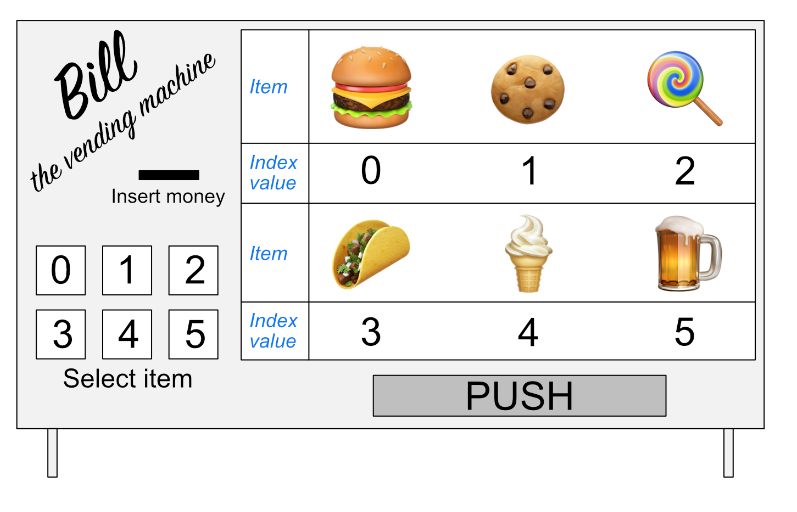
\includegraphics{./Figs/index.png}
\end{frame}

\begin{frame}{Ilustrim}
\protect\hypertarget{ilustrim-1}{}
\begin{itemize}
\item
  Makina automatike që përmban 6 artikuj.
\item
  Si Python, makina automatike përdor indekse për të zgjedhur artikujt.
\item
  Indeksi i parë është gjithmonë 0, dhe numri rritet me njësi.
\item
  Për të marrë një artikull nga makina automatike, duhet të përdorim
  indeksin e duhur.
\end{itemize}
\end{frame}

\begin{frame}[fragile]{Shembull me Makinë Automatike}
\protect\hypertarget{shembull-me-makinuxeb-automatike}{}
\begin{itemize}
\item
  Për të marrë një taco, do të zgjidhnit butonin 3.
\item
  Në Python, për të marrë një artikull nga një listë, përdorim indeksin
  përkatës:
\end{itemize}

\begin{Shaded}
\begin{Highlighting}[]
\NormalTok{  Bill[}\DecValTok{3}\NormalTok{]  }\CommentTok{\# Kthen "Taco"}
\end{Highlighting}
\end{Shaded}
\end{frame}

\begin{frame}[fragile]{Gjetja e Gjatësisë së Një Liste}
\protect\hypertarget{gjetja-e-gjatuxebsisuxeb-suxeb-njuxeb-liste}{}
\begin{itemize}
\tightlist
\item
  Për të marrë gjatësinë e një liste, përdorim funksionin
  \texttt{len()}:
\end{itemize}

\begin{Shaded}
\begin{Highlighting}[]
\NormalTok{  qytete }\OperatorTok{=}\NormalTok{ [}\StringTok{"Tiranë"}\NormalTok{, }\StringTok{"Durrës"}\NormalTok{, }\StringTok{"Shkodër"}\NormalTok{, }\StringTok{"Vlorë"}\NormalTok{]}
  \BuiltInTok{len}\NormalTok{(qytete)  }\CommentTok{\# Kthen 4}
\end{Highlighting}
\end{Shaded}
\end{frame}

\begin{frame}[fragile]{Përdorimi i len() për të gjetur vlerën e fundit
të një liste}
\protect\hypertarget{puxebrdorimi-i-len-puxebr-tuxeb-gjetur-vleruxebn-e-fundit-tuxeb-njuxeb-liste}{}
\begin{itemize}
\item
  Duke përdorur \textbf{len()}, mund të gjejmë indeksin e fundit të një
  liste.
\item
  Indeksi i fundit është gjithmonë \textbf{len(qytete) - 1}:
\end{itemize}

\begin{Shaded}
\begin{Highlighting}[]
\NormalTok{qytete[}\BuiltInTok{len}\NormalTok{(qytete) }\OperatorTok{{-}} \DecValTok{1}\NormalTok{]  }\CommentTok{\# Kthen "Vlorë"}
\end{Highlighting}
\end{Shaded}
\end{frame}

\begin{frame}[fragile]{Përdorimi i len() për të gjetur vlerën e fundit
të një liste}
\protect\hypertarget{puxebrdorimi-i-len-puxebr-tuxeb-gjetur-vleruxebn-e-fundit-tuxeb-njuxeb-liste-1}{}
\begin{itemize}
\tightlist
\item
  Për të marrë vlerën e fundit, përdorim indeksin -1:
\end{itemize}

\begin{Shaded}
\begin{Highlighting}[]
\NormalTok{qytete[}\OperatorTok{{-}}\DecValTok{1}\NormalTok{]  }\CommentTok{\# Kthen "Vlorë"}
\end{Highlighting}
\end{Shaded}
\end{frame}

\begin{frame}[fragile]{Kujdes me Indekset Jashtë Kufijve}
\protect\hypertarget{kujdes-me-indekset-jashtuxeb-kufijve-1}{}
\begin{itemize}
\tightlist
\item
  Nëse përdorim një indeks që është jashtë kufijve të listës, do të
  merrni një IndexError.
\end{itemize}

\begin{Shaded}
\begin{Highlighting}[]
\NormalTok{qytete[}\DecValTok{4}\NormalTok{]  }\CommentTok{\# Kthen "IndexError: list index out of range"}
\end{Highlighting}
\end{Shaded}
\end{frame}

\begin{frame}[fragile]{Përdorimi i Indeksimit Negativ}
\protect\hypertarget{puxebrdorimi-i-indeksimit-negativ}{}
\begin{itemize}
\item
  Indeksimi negativ na lejon të marrim elementë nga fundi i një liste.
\item
  Indeksi \texttt{-1} jep vlerën e fundit, ndërsa indekset me vlera më
  të mëdha negative shkojnë drejt fillimit të listës:
\end{itemize}

\begin{Shaded}
\begin{Highlighting}[]
\NormalTok{  qytete }\OperatorTok{=}\NormalTok{ [}\StringTok{"Tiranë"}\NormalTok{, }\StringTok{"Durrës"}\NormalTok{, }\StringTok{"Shkodër"}\NormalTok{, }\StringTok{"Vlorë"}\NormalTok{]}
\NormalTok{  qytete[}\OperatorTok{{-}}\DecValTok{1}\NormalTok{]  }\CommentTok{\# Kthen "Vlorë"}
\NormalTok{  qytete[}\OperatorTok{{-}}\DecValTok{2}\NormalTok{]  }\CommentTok{\# Kthen "Shkodër"}
\end{Highlighting}
\end{Shaded}
\end{frame}

\begin{frame}[fragile]{Kujdes me Indekset Negativë}
\protect\hypertarget{kujdes-me-indekset-negativuxeb}{}
Edhe pse indeksimi negativ është i dobishëm, përdorimi i një indeksi
jashtë kufijve shkakton \textbf{IndexError}:

\begin{Shaded}
\begin{Highlighting}[]
\NormalTok{qytete[}\OperatorTok{{-}}\DecValTok{5}\NormalTok{]  }\CommentTok{\# Kthen "IndexError: list index out of range"}
\end{Highlighting}
\end{Shaded}
\end{frame}

\begin{frame}[fragile]{Shembuj të Tjerë të Indeksimit Negativ}
\protect\hypertarget{shembuj-tuxeb-tjeruxeb-tuxeb-indeksimit-negativ}{}
\begin{itemize}
\tightlist
\item
  Indeksi \textbf{-len(qytete)} jep vlerën e parë në listë:
\end{itemize}

\begin{Shaded}
\begin{Highlighting}[]
\NormalTok{qytete[}\OperatorTok{{-}}\BuiltInTok{len}\NormalTok{(qytete)]  }\CommentTok{\# Kthen "Tiranë"}
\end{Highlighting}
\end{Shaded}
\end{frame}

\begin{frame}{Listat janë të Ndryshueshme}
\protect\hypertarget{listat-januxeb-tuxeb-ndryshueshme}{}
\begin{itemize}
\item
  Një nga avantazhet e listave është se ato mund të ndryshohen pasi të
  krijohen.
\item
  Për të ndryshuar një vlerë në një listë, përdorim indeksin për të
  përcaktuar pozicionin e vlerës që duam të ndryshojmë.
\end{itemize}
\end{frame}

\begin{frame}[fragile]{Shembull: Listë e Qyteteve Shqiptare}
\protect\hypertarget{shembull-listuxeb-e-qyteteve-shqiptare}{}
\begin{itemize}
\tightlist
\item
  Le të krijojmë një listë që përfshin qytetet kryesore shqiptare:
\end{itemize}

\begin{Shaded}
\begin{Highlighting}[]
\NormalTok{  qytete }\OperatorTok{=}\NormalTok{ [}\StringTok{"Tiranë"}\NormalTok{, }\StringTok{"Durrës"}\NormalTok{, }\StringTok{"Shkodër"}\NormalTok{, }\StringTok{"Vlorë"}\NormalTok{]}
\end{Highlighting}
\end{Shaded}
\end{frame}

\begin{frame}[fragile]{Shembull: Listë e Qyteteve Shqiptare}
\protect\hypertarget{shembull-listuxeb-e-qyteteve-shqiptare-1}{}
\begin{itemize}
\tightlist
\item
  Për të ndryshuar qytetin e tretë në listë, përdorim indeksin përkatës:
\end{itemize}

\begin{Shaded}
\begin{Highlighting}[]
\NormalTok{qytete[}\DecValTok{2}\NormalTok{] }\OperatorTok{=} \StringTok{"Elbasan"}  \CommentTok{\# Ndryshon Shkodrën në Elbasan}
\end{Highlighting}
\end{Shaded}
\end{frame}

\begin{frame}[fragile]{Shembull: Listë e Qyteteve Shqiptare}
\protect\hypertarget{shembull-listuxeb-e-qyteteve-shqiptare-2}{}
Pas modifikimit të vlerës, mund të printojmë listën për të parë
ndryshimin:

\begin{Shaded}
\begin{Highlighting}[]
\BuiltInTok{print}\NormalTok{(qytete)  }\CommentTok{\# Kthen ["Tiranë", "Durrës", "Elbasan", "Vlorë"]}
\end{Highlighting}
\end{Shaded}
\end{frame}

\begin{frame}[fragile]{Përdorimi i Indekseve për Modifikim}
\protect\hypertarget{puxebrdorimi-i-indekseve-puxebr-modifikim}{}
\begin{itemize}
\tightlist
\item
  Indeksi i parë është gjithmonë 0, kështu që për të ndryshuar vlerën e
  parë, përdorim indeksin 0:
\end{itemize}

\begin{Shaded}
\begin{Highlighting}[]
\NormalTok{qytete[}\DecValTok{0}\NormalTok{] }\OperatorTok{=} \StringTok{"Korçë"}  \CommentTok{\# Ndryshon Tiranën në Korçë}
\end{Highlighting}
\end{Shaded}
\end{frame}

\begin{frame}[fragile]{Përdorimi i Indekseve për Modifikim}
\protect\hypertarget{puxebrdorimi-i-indekseve-puxebr-modifikim-1}{}
\begin{itemize}
\tightlist
\item
  Për të ndryshuar vlerën e fundit, përdorim indeksin -1:
\end{itemize}

\begin{Shaded}
\begin{Highlighting}[]
\NormalTok{qytete[}\OperatorTok{{-}}\DecValTok{1}\NormalTok{] }\OperatorTok{=} \StringTok{"Sarandë"}  \CommentTok{\# Ndryshon Vlorën në Sarandë}
\end{Highlighting}
\end{Shaded}
\end{frame}

\begin{frame}[fragile]{Përdorimi i Indekseve për Modifikim}
\protect\hypertarget{puxebrdorimi-i-indekseve-puxebr-modifikim-2}{}
Pas modifikimit, printoni listën për të verifikuar ndryshimin:

\begin{Shaded}
\begin{Highlighting}[]
\BuiltInTok{print}\NormalTok{(qytete)  }\CommentTok{\# Kthen ["Korçë", "Durrës", "Elbasan", "Sarandë"]}
\end{Highlighting}
\end{Shaded}
\end{frame}

\begin{frame}{Kujdes me Indekset Jashtë Kufijve}
\protect\hypertarget{kujdes-me-indekset-jashtuxeb-kufijve-2}{}
Nëse përdorni një indeks që është jashtë kufijve të listës, do të marrim
një \textbf{IndexError}.
\end{frame}

\begin{frame}[fragile]{Shembuj të Tjerë të Modifikimit}
\protect\hypertarget{shembuj-tuxeb-tjeruxeb-tuxeb-modifikimit}{}
Për të ndryshuar vlerat e mesme, përdorim indeksin përkatës:

\begin{Shaded}
\begin{Highlighting}[]
\NormalTok{qytete[}\DecValTok{1}\NormalTok{] }\OperatorTok{=} \StringTok{"Fier"}  \CommentTok{\# Ndryshon Durrësin në Fier}
\end{Highlighting}
\end{Shaded}
\end{frame}

\begin{frame}[fragile]{Përdorimi i Indekseve për Modifikim}
\protect\hypertarget{puxebrdorimi-i-indekseve-puxebr-modifikim-3}{}
Pas modifikimit, printoni listën për të verifikuar ndryshimin:

\begin{Shaded}
\begin{Highlighting}[]
\BuiltInTok{print}\NormalTok{(qytete)  }\CommentTok{\# Kthen ["Korçë", "Fier", "Elbasan", "Sarandë"]}
\end{Highlighting}
\end{Shaded}
\end{frame}

\begin{frame}[fragile]{Lista që Përmban Tipa të Ndryshëm të Dhënave}
\protect\hypertarget{lista-quxeb-puxebrmban-tipa-tuxeb-ndryshuxebm-tuxeb-dhuxebnave}{}
\begin{itemize}
\item
  Një nga përfitimet e një liste është se ajo mund të përmbajë lloje të
  ndryshme të dhënash në të njëjtin koleksion.
\item
  Për shembull, le të krijojmë një listë që përmban emrin e një qyteti
  shqiptar, kodin e postës, koordinatat gjeografike, dhe një atribut
  tjetër.
\end{itemize}

\begin{Shaded}
\begin{Highlighting}[]
\NormalTok{  city\_name }\OperatorTok{=} \StringTok{"Tiranë"}
\NormalTok{  postal\_code }\OperatorTok{=} \DecValTok{1001}
\NormalTok{  city\_lat }\OperatorTok{=} \FloatTok{41.3275}
\NormalTok{  city\_lon }\OperatorTok{=} \FloatTok{19.8189}
\NormalTok{  major\_landmark }\OperatorTok{=} \StringTok{"Sheshi Skënderbej"}
\end{Highlighting}
\end{Shaded}
\end{frame}

\begin{frame}[fragile]{Lista që Përmban Tipa të Ndryshëm të Dhënave}
\protect\hypertarget{lista-quxeb-puxebrmban-tipa-tuxeb-ndryshuxebm-tuxeb-dhuxebnave-1}{}
\begin{itemize}
\tightlist
\item
  Kombinojmë këto variabla në një listë që përmban lloje të ndryshme të
  dhënash:
\end{itemize}

\begin{Shaded}
\begin{Highlighting}[]
\NormalTok{city\_info }\OperatorTok{=}\NormalTok{ [city\_name, postal\_code, city\_lat, city\_lon, major\_landmark]}
\end{Highlighting}
\end{Shaded}
\end{frame}

\begin{frame}[fragile]{Kontrollimi i Llojit të Listës}
\protect\hypertarget{kontrollimi-i-llojit-tuxeb-listuxebs}{}
\begin{itemize}
\tightlist
\item
  Përdorim \textbf{type()} për të konfirmuar se është një listë:
\end{itemize}

\begin{Shaded}
\begin{Highlighting}[]
\BuiltInTok{type}\NormalTok{(city\_info)  }\CommentTok{\# Kthen "list"}
\end{Highlighting}
\end{Shaded}
\end{frame}

\begin{frame}[fragile]{Kontrollimi i Llojit të Listës}
\protect\hypertarget{kontrollimi-i-llojit-tuxeb-listuxebs-1}{}
\begin{itemize}
\tightlist
\item
  Për të kontrolluar llojet e të dhënave brenda listës, përdorim indekse
  të ndryshme:
\end{itemize}

\begin{Shaded}
\begin{Highlighting}[]
\BuiltInTok{type}\NormalTok{(city\_info[}\DecValTok{0}\NormalTok{])  }\CommentTok{\# Kthen "str"}
\BuiltInTok{type}\NormalTok{(city\_info[}\DecValTok{1}\NormalTok{])  }\CommentTok{\# Kthen "int"}
\BuiltInTok{type}\NormalTok{(city\_info[}\DecValTok{2}\NormalTok{])  }\CommentTok{\# Kthen "float"}
\end{Highlighting}
\end{Shaded}
\end{frame}

\begin{frame}{Kujdes me Përzierjen e Llojeve të Dhënave}
\protect\hypertarget{kujdes-me-puxebrzierjen-e-llojeve-tuxeb-dhuxebnave}{}
\begin{itemize}
\item
  Edhe pse një listë mund të përmbajë lloje të ndryshme, mund të jetë
  problematike në disa raste.
\item
  Rekomandohet që listat të kenë lloje të ngjashme për të shmangur
  probleme në analizat e të dhënave.
\end{itemize}
\end{frame}

\begin{frame}[fragile]{Shtimi dhe Heqja e Vlerave nga Listat}
\protect\hypertarget{shtimi-dhe-heqja-e-vlerave-nga-listat}{}
\begin{itemize}
\tightlist
\item
  Le të kemi një listë me emrat e disa qyteteve kryesore në Shqipëri:
\end{itemize}

\begin{Shaded}
\begin{Highlighting}[]
\NormalTok{  qytete }\OperatorTok{=}\NormalTok{ [}\StringTok{"Tiranë"}\NormalTok{, }\StringTok{"Durrës"}\NormalTok{, }\StringTok{"Vlorë"}\NormalTok{, }\StringTok{"Shkodër"}\NormalTok{]}
\end{Highlighting}
\end{Shaded}
\end{frame}

\begin{frame}[fragile]{Heqja e Vlerave}
\protect\hypertarget{heqja-e-vlerave}{}
\begin{itemize}
\tightlist
\item
  Për të hequr vlerën e parë nga lista, përdorni del me indeksin e
  duhur:
\end{itemize}

\begin{Shaded}
\begin{Highlighting}[]
\KeywordTok{del}\NormalTok{ qytete[}\DecValTok{0}\NormalTok{]  }\CommentTok{\# Heq "Tiranë"}
\BuiltInTok{print}\NormalTok{(qytete)  }\CommentTok{\# Kthen [\textquotesingle{}Durrës\textquotesingle{}, \textquotesingle{}Vlorë\textquotesingle{}, \textquotesingle{}Shkodër\textquotesingle{}]}
\end{Highlighting}
\end{Shaded}
\end{frame}

\begin{frame}[fragile]{Heqja e Vlerave}
\protect\hypertarget{heqja-e-vlerave-1}{}
\begin{itemize}
\tightlist
\item
  Metoda \textbf{remove()} mund të përdoret për të hequr një element
  specifik nga lista pa përdorur indeksin:
\end{itemize}

\begin{Shaded}
\begin{Highlighting}[]
\NormalTok{qytete.remove(}\StringTok{"Durrës"}\NormalTok{)  }\CommentTok{\# Heq "Durrës"}
\BuiltInTok{print}\NormalTok{(qytete)  }\CommentTok{\# Kthen [\textquotesingle{}Vlorë\textquotesingle{}, \textquotesingle{}Shkodër\textquotesingle{}]}
\end{Highlighting}
\end{Shaded}
\end{frame}

\begin{frame}[fragile]{Shtimi i Vlerave}
\protect\hypertarget{shtimi-i-vlerave}{}
\begin{itemize}
\tightlist
\item
  Për të shtuar vlera në fund të listës, përdorni append():
\end{itemize}

\begin{Shaded}
\begin{Highlighting}[]
\NormalTok{qytete.append(}\StringTok{"Elbasan"}\NormalTok{)}
\NormalTok{qytete.append(}\StringTok{"Korçë"}\NormalTok{)}
\BuiltInTok{print}\NormalTok{(qytete)  }\CommentTok{\# Kthen [\textquotesingle{}Vlorë\textquotesingle{}, \textquotesingle{}Shkodër\textquotesingle{}, \textquotesingle{}Elbasan\textquotesingle{}, \textquotesingle{}Korçë\textquotesingle{}]}
\end{Highlighting}
\end{Shaded}
\end{frame}

\begin{frame}[fragile]{Kufizimet e Metodës append në Python}
\protect\hypertarget{kufizimet-e-metoduxebs-append-nuxeb-python}{}
\begin{itemize}
\item
  Metoda \texttt{append()} është projektuar për listat, duke shtuar
  elementë në fund të një liste.
\item
  Nuk ka kuptim ta përdorim për lloje të tjera të dhënash si
  \texttt{int}, sepse një numër i plotë nuk është një koleksion.
\end{itemize}
\end{frame}

\begin{frame}[fragile]{Shembull me Indeksimin e Një Liste}
\protect\hypertarget{shembull-me-indeksimin-e-njuxeb-liste}{}
\begin{itemize}
\tightlist
\item
  Le të kemi një listë me emrat e disa qyteteve shqiptare:
\end{itemize}

\begin{Shaded}
\begin{Highlighting}[]
\NormalTok{  qytete }\OperatorTok{=}\NormalTok{ [}\StringTok{"Tiranë"}\NormalTok{, }\StringTok{"Durrës"}\NormalTok{, }\StringTok{"Vlorë"}\NormalTok{, }\StringTok{"Shkodër"}\NormalTok{]}
\end{Highlighting}
\end{Shaded}
\end{frame}

\begin{frame}[fragile]{Kur gjatësia e listës llogaritet, rezultati është
një int:}
\protect\hypertarget{kur-gjatuxebsia-e-listuxebs-llogaritet-rezultati-uxebshtuxeb-njuxeb-int}{}
\begin{Shaded}
\begin{Highlighting}[]
\NormalTok{qytete\_length }\OperatorTok{=} \BuiltInTok{len}\NormalTok{(qytete)  }\CommentTok{\# Kthen 4}
\end{Highlighting}
\end{Shaded}
\end{frame}

\begin{frame}[fragile]{Çfarë ndodh kur përdorim append me int?}
\protect\hypertarget{uxe7faruxeb-ndodh-kur-puxebrdorim-append-me-int}{}
\begin{itemize}
\item
  Duke qenë se int është një lloj i dhënash që përfaqëson vlera të
  plota, nuk mund të shtojmë vlera në mënyrë sekuenciale si te një
  listë.
\item
  Përpjekja për të përdorur \textbf{append()} me një int shkakton një
  \textbf{AttributeError}:
\end{itemize}

\begin{Shaded}
\begin{Highlighting}[]
\NormalTok{qytete\_length.append(}\DecValTok{1}\NormalTok{)  }\CommentTok{\# Kthen "AttributeError: \textquotesingle{}int\textquotesingle{} object has no attribute \textquotesingle{}append\textquotesingle{}"}
\end{Highlighting}
\end{Shaded}
\end{frame}

\begin{frame}[fragile]{Zgjidhje për Shtimin e Vlerave të Tipit int}
\protect\hypertarget{zgjidhje-puxebr-shtimin-e-vlerave-tuxeb-tipit-int}{}
\begin{itemize}
\tightlist
\item
  Për të rritur një int, përdorim operacionet aritmetike të zakonshme:
\end{itemize}

\begin{Shaded}
\begin{Highlighting}[]
\NormalTok{qytete\_length }\OperatorTok{+=} \DecValTok{1}  \CommentTok{\# Rrit vlerën me 1}
\end{Highlighting}
\end{Shaded}
\end{frame}

\begin{frame}[fragile]{Numërimi i Një Vlere në Listë}
\protect\hypertarget{numuxebrimi-i-njuxeb-vlere-nuxeb-listuxeb}{}
\begin{itemize}
\item
  Përdorim metodën \texttt{count()} për të parë sa herë një vlerë
  shfaqet në një listë.
\item
  Shembull:
\end{itemize}

\begin{Shaded}
\begin{Highlighting}[]
\NormalTok{  qytete }\OperatorTok{=}\NormalTok{ [}\StringTok{"Tiranë"}\NormalTok{, }\StringTok{"Durrës"}\NormalTok{, }\StringTok{"Vlorë"}\NormalTok{, }\StringTok{"Shkodër"}\NormalTok{, }\StringTok{"Tiranë"}\NormalTok{]}
\NormalTok{  qytete.count(}\StringTok{"Tiranë"}\NormalTok{)  }\CommentTok{\# Kthen 2}
\end{Highlighting}
\end{Shaded}
\end{frame}

\begin{frame}[fragile]{Gjetja e Indeksit të Një Vlere}
\protect\hypertarget{gjetja-e-indeksit-tuxeb-njuxeb-vlere}{}
\begin{itemize}
\item
  Metoda \emph{index()} na lejon të gjejmë indeksin e parë ku shfaqet
  një vlerë.
\item
  Shembull:
\end{itemize}

\begin{Shaded}
\begin{Highlighting}[]
\NormalTok{qytete.index(}\StringTok{"Vlorë"}\NormalTok{)  }\CommentTok{\# Kthen 2}
\end{Highlighting}
\end{Shaded}
\end{frame}

\begin{frame}[fragile]{Kthimi i Renditjes së Një Liste}
\protect\hypertarget{kthimi-i-renditjes-suxeb-njuxeb-liste}{}
\begin{itemize}
\tightlist
\item
  Për të kthyer renditjen e listës, përdorim metodën \emph{reverse()}:
\end{itemize}

\begin{Shaded}
\begin{Highlighting}[]
\NormalTok{qytete.reverse()}
\BuiltInTok{print}\NormalTok{(qytete)  }\CommentTok{\# Kthen [\textquotesingle{}Shkodër\textquotesingle{}, \textquotesingle{}Vlorë\textquotesingle{}, \textquotesingle{}Durrës\textquotesingle{}, \textquotesingle{}Tiranë\textquotesingle{}]}
\end{Highlighting}
\end{Shaded}
\end{frame}

\begin{frame}[fragile]{Kthimi i Renditjes së Një Liste}
\protect\hypertarget{kthimi-i-renditjes-suxeb-njuxeb-liste-1}{}
Kujdes kur përdorni \emph{reverse()} dhe mos caktoni rezultatin në të
njëjtën listë, pasi kjo do të shkaktojë një None:

\begin{Shaded}
\begin{Highlighting}[]
\NormalTok{qytete }\OperatorTok{=}\NormalTok{ qytete.reverse()  }\CommentTok{\# Gabim! Kthen None dhe fshin përmbajtjen e listës}
\end{Highlighting}
\end{Shaded}
\end{frame}

\begin{frame}[fragile]{Renditja e Një Liste Alfabetikisht}
\protect\hypertarget{renditja-e-njuxeb-liste-alfabetikisht}{}
\begin{itemize}
\tightlist
\item
  Metoda \emph{sort()} mund të përdoret për të renditur listën në mënyrë
  alfabetike:
\end{itemize}

\begin{Shaded}
\begin{Highlighting}[]
\NormalTok{qytete.sort()}
\BuiltInTok{print}\NormalTok{(qytete)  }\CommentTok{\# Kthen [\textquotesingle{}Durrës\textquotesingle{}, \textquotesingle{}Shkodër\textquotesingle{}, \textquotesingle{}Tiranë\textquotesingle{}, \textquotesingle{}Vlorë\textquotesingle{}]}
\end{Highlighting}
\end{Shaded}
\end{frame}

\begin{frame}[fragile]{Renditja e Një Liste Alfabetikisht}
\protect\hypertarget{renditja-e-njuxeb-liste-alfabetikisht-1}{}
\begin{itemize}
\tightlist
\item
  Për të shmangur gabimet, mos caktoni rezultatin e \emph{sort()} në
  listën e njëjtë, pasi kjo do të shkaktojë një None:
\end{itemize}

\begin{Shaded}
\begin{Highlighting}[]
\NormalTok{qytete }\OperatorTok{=}\NormalTok{ qytete.sort()  }\CommentTok{\# Gabim! Kthen None dhe fshin përmbajtjen e listës}
\end{Highlighting}
\end{Shaded}
\end{frame}

\begin{frame}[fragile]{Definimi i Variablave me Tipa të Ndryshëm}
\protect\hypertarget{definimi-i-variablave-me-tipa-tuxeb-ndryshuxebm}{}
\begin{itemize}
\tightlist
\item
  Në këtë shembull, kemi pesë variabla që përfaqësojnë të dhëna të
  ndryshme për një qytet ose një stacion:
\end{itemize}

\begin{Shaded}
\begin{Highlighting}[]
\NormalTok{  station\_name }\OperatorTok{=} \StringTok{"Tiranë"}
\NormalTok{  station\_id }\OperatorTok{=} \DecValTok{1001}
\NormalTok{  station\_lat }\OperatorTok{=} \FloatTok{41.3275}
\NormalTok{  station\_lon }\OperatorTok{=} \FloatTok{19.8189}
\NormalTok{  station\_type }\OperatorTok{=} \StringTok{"Kryeqytet"}
\end{Highlighting}
\end{Shaded}
\end{frame}

\begin{frame}[fragile]{Kontrollimi i Llojeve të Të Dhënave}
\protect\hypertarget{kontrollimi-i-llojeve-tuxeb-tuxeb-dhuxebnave}{}
\begin{itemize}
\tightlist
\item
  Përdorim funksionin \emph{type()} për të kontrolluar llojin e një
  variabli:
\end{itemize}

\begin{Shaded}
\begin{Highlighting}[]
\BuiltInTok{type}\NormalTok{(station\_name)  }\CommentTok{\# Kthen "str"}
\BuiltInTok{type}\NormalTok{(station\_id)  }\CommentTok{\# Kthen "int"}
\BuiltInTok{type}\NormalTok{(station\_lat)  }\CommentTok{\# Kthen "float"}
\end{Highlighting}
\end{Shaded}
\end{frame}

\begin{frame}[fragile]{Gabime të Zakonshme me Llojet e Të Dhënave}
\protect\hypertarget{gabime-tuxeb-zakonshme-me-llojet-e-tuxeb-dhuxebnave}{}
\begin{itemize}
\tightlist
\item
  Nëse përpiqeni të bashkoni një varg me një numër të plotë, do të
  shkaktoni një TypeError:
\end{itemize}

\begin{Shaded}
\begin{Highlighting}[]
\NormalTok{station\_name }\OperatorTok{+}\NormalTok{ station\_id  }\CommentTok{\# Kthen "TypeError: can only concatenate str (not \textquotesingle{}int\textquotesingle{}) to str"}
\end{Highlighting}
\end{Shaded}
\end{frame}

\begin{frame}[fragile]{Konvertimi i Të Dhënave për Përputhshmëri}
\protect\hypertarget{konvertimi-i-tuxeb-dhuxebnave-puxebr-puxebrputhshmuxebri}{}
\begin{itemize}
\tightlist
\item
  Për të kombinuar një varg me një numër të plotë, duhet të konvertojmë
  numrin në një varg duke përdorur funksionin \textbf{str()}:
\end{itemize}

\begin{Shaded}
\begin{Highlighting}[]
\NormalTok{station\_id\_str }\OperatorTok{=} \BuiltInTok{str}\NormalTok{(station\_id)}
\NormalTok{station\_name }\OperatorTok{+}\NormalTok{ station\_id\_str  }\CommentTok{\# Kthen "Tiranë1001"}
\end{Highlighting}
\end{Shaded}
\end{frame}

\begin{frame}[fragile]{Konvertimi i Të Dhënave për Përputhshmëri}
\protect\hypertarget{konvertimi-i-tuxeb-dhuxebnave-puxebr-puxebrputhshmuxebri-1}{}
\begin{itemize}
\tightlist
\item
  Në mënyrë të ngjashme, mund të konvertojmë një varg ose një numër
  dhjetor në një numër të plotë duke përdorur \emph{int()}, ose në një
  numër dhjetor duke përdorur \emph{float()}: python
\end{itemize}

\begin{Shaded}
\begin{Highlighting}[]
\BuiltInTok{float}\NormalTok{(}\StringTok{"3.14"}\NormalTok{)  }\CommentTok{\# Kthen 3.14 (numër dhjetor)}
\BuiltInTok{int}\NormalTok{(}\StringTok{"1001"}\NormalTok{)  }\CommentTok{\# Kthen 1001 (numër i plotë)}
\end{Highlighting}
\end{Shaded}
\end{frame}

\hypertarget{manipulimi-i-tekstit}{%
\section*{Manipulimi i tekstit}\label{manipulimi-i-tekstit}}
\addcontentsline{toc}{section}{Manipulimi i tekstit}

\begin{frame}[fragile]{Kombinimi i Tekstit dhe Numrave në Python}
\protect\hypertarget{kombinimi-i-tekstit-dhe-numrave-nuxeb-python}{}
\begin{itemize}
\item
  Një mënyrë e zakonshme për të kombinuar vargje dhe numra është
  përdorimi i operatorit të shtimit \texttt{+}.
\item
  Në këtë shembull, ne kombinojmë një emër qyteti dhe një kod postar për
  të krijuar një varg të ri:
\end{itemize}

\begin{Shaded}
\begin{Highlighting}[]
\NormalTok{  city\_name }\OperatorTok{=} \StringTok{"Tiranë"}
\NormalTok{  postal\_code }\OperatorTok{=} \DecValTok{1001}
\NormalTok{  city\_info }\OperatorTok{=}\NormalTok{ city\_name }\OperatorTok{+} \StringTok{" {-} "} \OperatorTok{+} \BuiltInTok{str}\NormalTok{(postal\_code)}
\NormalTok{  city\_info  }\CommentTok{\# Kthen "Tiranë {-} 1001"}
\end{Highlighting}
\end{Shaded}
\end{frame}

\begin{frame}[fragile]{Përdorimi i F-Strings për Manipulimin e Tekstit}
\protect\hypertarget{puxebrdorimi-i-f-strings-puxebr-manipulimin-e-tekstit}{}
\begin{itemize}
\item
  Një metodë më e avancuar për të bashkuar vargjet dhe numrat është
  përdorimi i f-strings.
\item
  F-strings lejojnë futjen e variablave brenda vargjeve në mënyrë
  dinamike.
\item
  Shembull:
\end{itemize}

\begin{Shaded}
\begin{Highlighting}[]
\NormalTok{temp }\OperatorTok{=} \FloatTok{18.56789876}
\NormalTok{f\_string\_example }\OperatorTok{=} \SpecialStringTok{f"Temperatura në }\SpecialCharTok{\{}\NormalTok{city\_name}\SpecialCharTok{\}}\SpecialStringTok{ është }\SpecialCharTok{\{}\NormalTok{temp}\SpecialCharTok{:.2f\}}\SpecialStringTok{ gradë Celsius"}
\NormalTok{f\_string\_example  }\CommentTok{\# Kthen "Temperatura në Tiranë është 18.57 gradë Celsius"}
\end{Highlighting}
\end{Shaded}
\end{frame}

\begin{frame}{Shpjegimi i F-Strings}
\protect\hypertarget{shpjegimi-i-f-strings}{}
\begin{itemize}
\item
  Përdorni shkronjën f para vargut për të krijuar një f-string.
\item
  Variablat mund të futen brenda vargut duke përdorur kllapat \{\}.
\end{itemize}
\end{frame}

\begin{frame}[fragile]{Shpjegimi i F-Strings}
\protect\hypertarget{shpjegimi-i-f-strings-1}{}
\begin{itemize}
\tightlist
\item
  Është gjithashtu e mundur të përdorni formatime për të rregulluar
  precizionin e numrave:
\end{itemize}

\begin{Shaded}
\begin{Highlighting}[]
\NormalTok{f\_string\_example }\OperatorTok{=} \SpecialStringTok{f"Temperatura është }\SpecialCharTok{\{}\NormalTok{temp}\SpecialCharTok{:.2f\}}\SpecialStringTok{ gradë Celsius"}
\end{Highlighting}
\end{Shaded}
\end{frame}

\begin{frame}[fragile]{Teknikat e Tjera për Manipulimin e Tekstit}
\protect\hypertarget{teknikat-e-tjera-puxebr-manipulimin-e-tekstit}{}
\begin{itemize}
\item
  Përveç f-strings, ekzistojnë edhe metodat \textbf{.format()} dhe
  \textbf{\%} për manipulimin e tekstit.
\item
  Megjithatë, f-strings janë metoda e rekomanduar për shkak të
  thjeshtësisë dhe fleksibilitetit.
\item
  Shembull me \textbf{.format()}:
\end{itemize}

\begin{Shaded}
\begin{Highlighting}[]
\NormalTok{format\_example }\OperatorTok{=} \StringTok{"Temperatura në }\SpecialCharTok{\{\}}\StringTok{ është }\SpecialCharTok{\{:.2f\}}\StringTok{ gradë"}\NormalTok{.}\BuiltInTok{format}\NormalTok{(city\_name, temp)}
\NormalTok{format\_example  }\CommentTok{\# Kthen "Temperatura në Tiranë është 18.57 gradë"}
\end{Highlighting}
\end{Shaded}
\end{frame}

\begin{frame}[fragile]{Shembull me \% (më pak i rekomanduar):}
\protect\hypertarget{shembull-me-muxeb-pak-i-rekomanduar}{}
\begin{Shaded}
\begin{Highlighting}[]
\NormalTok{percent\_example }\OperatorTok{=} \StringTok{"Temperatura në }\SpecialCharTok{\%s}\StringTok{ është }\SpecialCharTok{\%.2f}\StringTok{ gradë"} \OperatorTok{\%}\NormalTok{ (city\_name, temp)}
\NormalTok{percent\_example  }\CommentTok{\# Kthen "Temperatura në Tiranë është 18.57 gradë"}
\end{Highlighting}
\end{Shaded}
\end{frame}

\begin{frame}[fragile]{Ndarja e Një Vargu me .split()}
\protect\hypertarget{ndarja-e-njuxeb-vargu-me-.split}{}
\begin{itemize}
\item
  Metoda \texttt{.split()} lejon ndarjen e një vargu bazuar në një
  karakter të caktuar.
\item
  Shembull:
\end{itemize}

\begin{Shaded}
\begin{Highlighting}[]
\NormalTok{  tekst }\OperatorTok{=} \StringTok{"Qytete: Tiranë, Durrës, Shkodër"}
\NormalTok{  pjese\_te\_ndara }\OperatorTok{=}\NormalTok{ tekst.split(}\StringTok{":"}\NormalTok{)}
\NormalTok{  pjese\_te\_ndara  }\CommentTok{\# Kthen [\textquotesingle{}Qytete\textquotesingle{}, \textquotesingle{} Tiranë, Durrës, Shkodër\textquotesingle{}]}
\end{Highlighting}
\end{Shaded}
\end{frame}

\begin{frame}[fragile]{Zëvendësimi i Një Fjale me .replace()}
\protect\hypertarget{zuxebvenduxebsimi-i-njuxeb-fjale-me-.replace}{}
\begin{itemize}
\item
  Metoda \emph{.replace()} lejon zëvendësimin e një fjale ose grupi
  karakteresh me një tjetër.
\item
  Shembull:
\end{itemize}

\begin{Shaded}
\begin{Highlighting}[]
\NormalTok{tekst\_ndryshuar }\OperatorTok{=}\NormalTok{ pjese\_te\_ndaura[}\DecValTok{1}\NormalTok{].replace(}\StringTok{"Tiranë"}\NormalTok{, }\StringTok{"Elbasan"}\NormalTok{)}
\NormalTok{tekst\_ndryshuar  }\CommentTok{\# Kthen \textquotesingle{} Elbasan, Durrës, Shkodër\textquotesingle{}}
\end{Highlighting}
\end{Shaded}
\end{frame}

\begin{frame}[fragile]{Prerja e Një Vargu për të Hequr Hapësirat e
Panevojshme}
\protect\hypertarget{prerja-e-njuxeb-vargu-puxebr-tuxeb-hequr-hapuxebsirat-e-panevojshme}{}
\begin{itemize}
\tightlist
\item
  Për të prerë karakteret e panevojshme nga fillimi ose fundi i një
  vargu, mund të përdorim metodën \emph{.strip()} ose të përdorim
  prerjen:
\end{itemize}

\begin{Shaded}
\begin{Highlighting}[]
\NormalTok{tekst\_prere }\OperatorTok{=}\NormalTok{ pjese\_te\_ndaura[}\DecValTok{1}\NormalTok{][}\DecValTok{1}\NormalTok{:]  }\CommentTok{\# Hiq hapësirën në fillim}
\NormalTok{tekst\_prere.strip()  }\CommentTok{\# Hiq hapësirat nga fillimi dhe fundi}
\end{Highlighting}
\end{Shaded}
\end{frame}

\begin{frame}[fragile]{Ndryshimi i Shkronjave me .upper() dhe .lower()}
\protect\hypertarget{ndryshimi-i-shkronjave-me-.upper-dhe-.lower}{}
\begin{itemize}
\tightlist
\item
  Për të ndryshuar të gjitha shkronjat në shkronja të mëdha, përdorni
  metodën \textbf{.upper()}:
\end{itemize}

\begin{Shaded}
\begin{Highlighting}[]
\NormalTok{tekst\_prere.upper()  }\CommentTok{\# Kthen \textquotesingle{}ELBASAN, DURRËS, SHKODËR\textquotesingle{}}
\end{Highlighting}
\end{Shaded}
\end{frame}

\begin{frame}[fragile]{Ndryshimi i Shkronjave me .upper() dhe .lower()}
\protect\hypertarget{ndryshimi-i-shkronjave-me-.upper-dhe-.lower-1}{}
\begin{itemize}
\tightlist
\item
  Për të kthyer të gjitha shkronjat në të vogla, përdorni metodën
  \textbf{.lower()}:
\end{itemize}

\begin{Shaded}
\begin{Highlighting}[]
\NormalTok{tekst\_prere.lower()  }\CommentTok{\# Kthen \textquotesingle{}elbasan, durrës, shkodër\textquotesingle{}}
\end{Highlighting}
\end{Shaded}
\end{frame}

\begin{frame}[fragile]{Ndryshimi i Shkronjave}
\protect\hypertarget{ndryshimi-i-shkronjave}{}
\begin{itemize}
\tightlist
\item
  Për të kapitalizuar vetëm shkronjën e parë, përdorni metodën
  \textbf{.capitalize()}:
\end{itemize}

\begin{Shaded}
\begin{Highlighting}[]
\NormalTok{tekst\_prere.capitalize()  }\CommentTok{\# Kthen \textquotesingle{}Elbasan, durrës, shkodër\textquotesingle{}}
\end{Highlighting}
\end{Shaded}
\end{frame}

\hypertarget{ciklet-for}{%
\section*{Ciklet ``For''}\label{ciklet-for}}
\addcontentsline{toc}{section}{Ciklet ``For''}

\begin{frame}{Ciklet ``For''}
\protect\hypertarget{ciklet-for-1}{}
\begin{itemize}
\item
  Ciklet ``for'' na lejojnë të përsërisim një bllok kodi disa herë, si
  iterimi mbi një listë dhe kryerja e një veprimi për çdo element.
\item
  Ato janë të dobishme për të automatizuar veprimet që përsëriten, për
  të shmangur gabimet dhe për të përmirësuar shkallëzueshmërinë e kodit.
\end{itemize}
\end{frame}

\begin{frame}[fragile]{Shembull i keq}
\protect\hypertarget{shembull-i-keq}{}
Si shembull, le të përpiqemi të marrim qytetet shqiptare me indeksim
manual:

\begin{Shaded}
\begin{Highlighting}[]
\NormalTok{qytete\_shqiptare }\OperatorTok{=}\NormalTok{ [}\StringTok{"Tiranë"}\NormalTok{, }\StringTok{"Durrës"}\NormalTok{, }\StringTok{"Shkodër"}\NormalTok{, }\StringTok{"Vlorë"}\NormalTok{]}
\NormalTok{qytete\_shqiptare[}\DecValTok{0}\NormalTok{]  }\CommentTok{\# \textquotesingle{}Tiranë\textquotesingle{}}
\NormalTok{qytete\_shqiptare[}\DecValTok{1}\NormalTok{]  }\CommentTok{\# \textquotesingle{}Durrës\textquotesingle{}}
\NormalTok{qytete\_shqiptare[}\DecValTok{2}\NormalTok{]  }\CommentTok{\# \textquotesingle{}Shkodër\textquotesingle{}}
\NormalTok{qytete\_shqiptare[}\DecValTok{3}\NormalTok{]  }\CommentTok{\# \textquotesingle{}Vlorë\textquotesingle{}}
\NormalTok{qytete\_shqiptare[}\DecValTok{4}\NormalTok{]  }\CommentTok{\# Kjo do të shkaktojë IndexError}
\end{Highlighting}
\end{Shaded}
\end{frame}

\begin{frame}{Shembulli i Keq}
\protect\hypertarget{shembulli-i-keq}{}
\begin{itemize}
\item
  Shembulli i përdorimit të indeksimit manual në listë
\item
  Mund të shkaktojë gabime IndexError dhe nuk është i shkallëzueshëm për
  lista të gjata.
\end{itemize}
\end{frame}

\begin{frame}{Përdorimi i ciklit ``for'' për të iteruar mbi një listë}
\protect\hypertarget{puxebrdorimi-i-ciklit-for-puxebr-tuxeb-iteruar-mbi-njuxeb-listuxeb}{}
\begin{itemize}
\item
  Kjo metodë është më fleksibël dhe e shkallëzueshme.
\item
  Shembulli i përdorimit të ciklit ``for'' për të iteruar mbi listën e
  qyteteve shqiptare
\end{itemize}
\end{frame}

\begin{frame}[fragile]{Përdorimi i ciklit ``for'' për të iteruar mbi një
listë}
\protect\hypertarget{puxebrdorimi-i-ciklit-for-puxebr-tuxeb-iteruar-mbi-njuxeb-listuxeb-1}{}
\begin{Shaded}
\begin{Highlighting}[]
\NormalTok{qytete\_shqiptare }\OperatorTok{=}\NormalTok{ [}\StringTok{"Tiranë"}\NormalTok{, }\StringTok{"Durrës"}\NormalTok{, }\StringTok{"Shkodër"}\NormalTok{, }\StringTok{"Vlorë"}\NormalTok{]}
\ControlFlowTok{for}\NormalTok{ qytet në qytete\_shqiptare:}
    \BuiltInTok{print}\NormalTok{(qytet)}
\end{Highlighting}
\end{Shaded}
\end{frame}

\begin{frame}[fragile]{Formati i For Loop në Python}
\protect\hypertarget{formati-i-for-loop-nuxeb-python}{}
\begin{itemize}
\tightlist
\item
  Struktura e përgjithshme e një ``for loop'' në Python është si më
  poshtë:
\end{itemize}

\begin{Shaded}
\begin{Highlighting}[]
\ControlFlowTok{for}\NormalTok{ variabli në koleksion:}
\NormalTok{    bëj diçka me variablin}
\end{Highlighting}
\end{Shaded}
\end{frame}

\begin{frame}{Aspektet Kyçe}
\protect\hypertarget{aspektet-kyuxe7e}{}
\begin{itemize}
\item
  Variabli:

  Mund të jetë çfarëdo emër që dëshirojmë.
\end{itemize}

Përdoret për të ruajtur vlerën aktuale nga koleksioni gjatë çdo iterimi.
\end{frame}

\begin{frame}{Përfundimi i Deklaratës For:}
\protect\hypertarget{puxebrfundimi-i-deklaratuxebs-for}{}
\begin{itemize}
\item
  Duhet të mbarojë me një ``:''.
\item
  Ky simbol tregon që pjesa e kodit që pason është pjesë e ``loop''.
\end{itemize}
\end{frame}

\begin{frame}{Indentimi}
\protect\hypertarget{indentimi}{}
\begin{itemize}
\item
  Kodi që duhet të ekzekutohet si pjesë e ``for loop'' duhet të jetë i
  vendosur me 4 hapësira nën deklaratën ``for''.
\item
  Ky indentim përcakton që ky kod është pjesë e ``loop''.
\end{itemize}
\end{frame}

\begin{frame}{Përfundimi i For Loop}
\protect\hypertarget{puxebrfundimi-i-for-loop}{}
\begin{itemize}
\item
  Nuk ka ndonjë fjalë speciale për të përfunduar ``loop''.
\item
  Mjafton të kthehesh tek indentimi normal për të treguar që ``loop'' ka
  përfunduar.
\end{itemize}
\end{frame}

\begin{frame}[fragile]{Shembull 1: Iterimi përmes një liste}
\protect\hypertarget{shembull-1-iterimi-puxebrmes-njuxeb-liste}{}
\begin{Shaded}
\begin{Highlighting}[]
\NormalTok{fruta }\OperatorTok{=}\NormalTok{ [}\StringTok{"mollë"}\NormalTok{, }\StringTok{"banane"}\NormalTok{, }\StringTok{"portokall"}\NormalTok{]}
\ControlFlowTok{for}\NormalTok{ frutë në fruta:}
    \BuiltInTok{print}\NormalTok{(frutë)}
\end{Highlighting}
\end{Shaded}

Ky ``loop'' iteron përmes një liste frutash dhe printon secilën.
\end{frame}

\begin{frame}[fragile]{Shembull 2: Përdorimi i range() për të
përsëritur}
\protect\hypertarget{shembull-2-puxebrdorimi-i-range-puxebr-tuxeb-puxebrsuxebritur}{}
\begin{Shaded}
\begin{Highlighting}[]
\NormalTok{për numër në }\BuiltInTok{range}\NormalTok{(}\DecValTok{5}\NormalTok{):}
    \BuiltInTok{print}\NormalTok{(numër)}
\end{Highlighting}
\end{Shaded}

Ky ``loop'' iteron nga 0 në 4, duke printuar secilin numër.
\end{frame}

\begin{frame}{Variabli For Loop në Python}
\protect\hypertarget{variabli-for-loop-nuxeb-python}{}
\begin{itemize}
\item
  Në Python, variabli që përdoret në një ``for loop'' është një variabël
  i zakonshëm.
\item
  Ai vazhdon të ekzistojë edhe pasi ``loop'' përfundon, duke marrë
  vlerën e fundit nga koleksioni i iteruar.
\end{itemize}
\end{frame}

\begin{frame}[fragile]{Shembull}
\protect\hypertarget{shembull-2}{}
\begin{Shaded}
\begin{Highlighting}[]
\NormalTok{kushte\_moti }\OperatorTok{=}\NormalTok{ [}
    \StringTok{"shi"}\NormalTok{,}
    \StringTok{"dëborë"}\NormalTok{,}
    \StringTok{"mjegull"}\NormalTok{,}
    \StringTok{"diell"}\NormalTok{,}
    \StringTok{"re"}\NormalTok{,}
    \StringTok{"breshër"}\NormalTok{,}
\NormalTok{]}

\NormalTok{për mot në kushte\_moti:}
    \BuiltInTok{print}\NormalTok{(mot)}
\end{Highlighting}
\end{Shaded}
\end{frame}

\begin{frame}{Shembull}
\protect\hypertarget{shembull-3}{}
\begin{itemize}
\item
  Ky ``for loop'' iteron mbi një listë të kushteve të motit dhe printon
  secilën.
\item
  Vlera e fundit që merr \textbf{moti} pas përfundimit të ``loop'' është
  ``breshër''.
\end{itemize}
\end{frame}

\begin{frame}[fragile]{Kontrollimi i Vlerës së Variablit pas Loop}
\protect\hypertarget{kontrollimi-i-vleruxebs-suxeb-variablit-pas-loop}{}
\begin{Shaded}
\begin{Highlighting}[]
\BuiltInTok{print}\NormalTok{(}\StringTok{"Pas loop{-}it, moti është"}\NormalTok{, mot)}
\end{Highlighting}
\end{Shaded}

\begin{itemize}
\item
  Ky kod tregon se çfarë vlerë ka variabli pas përfundimit të ``loop''.
\item
  Në këtë rast, pasi ``loop'' ka përfunduar, vlera e variablit mot është
  ``breshër''.
\end{itemize}
\end{frame}

\begin{frame}{For Loops Duke Përdorur Funksionin range() në Python}
\protect\hypertarget{for-loops-duke-puxebrdorur-funksionin-range-nuxeb-python}{}
\begin{itemize}
\item
  For loops në Python mund të përdoren për të iteruar mbi çdo listë
  vlerash.
\item
  Funksioni \textbf{range()} krijon një seri numrash për të përcaktuar
  sa herë duhet të përsëritet një ``for loop''.
\end{itemize}
\end{frame}

\begin{frame}{Sintaksa e range()}
\protect\hypertarget{sintaksa-e-range}{}
Sintaksa bazë për \textbf{range()} është:

\begin{itemize}
\item
  \textbf{range(stop):} Krijon një listë nga 0 deri në numrin ``stop -
  1''.
\item
  \textbf{range(start, stop, step):} Krijon një listë nga ``start'' deri
  në ``stop - 1'' me hapin e përcaktuar nga ``step''.
\end{itemize}
\end{frame}

\begin{frame}[fragile]{Shembull: For Loop me range(5)}
\protect\hypertarget{shembull-for-loop-me-range5}{}
\begin{Shaded}
\begin{Highlighting}[]
\NormalTok{për vlerë në }\BuiltInTok{range}\NormalTok{(}\DecValTok{5}\NormalTok{):}
    \BuiltInTok{print}\NormalTok{(vlerë)}
\end{Highlighting}
\end{Shaded}

\begin{itemize}
\item
  Ky ``for loop'' iteron 5 herë, duke printuar numrat nga 0 deri në 4.
\item
  Funksioni \textbf{range(5)} krijon një seri numrash nga 0 deri në 4.
\end{itemize}
\end{frame}

\begin{frame}[fragile]{Përdorimi i range() me Argumente të Përshtatura}
\protect\hypertarget{puxebrdorimi-i-range-me-argumente-tuxeb-puxebrshtatura}{}
\begin{itemize}
\tightlist
\item
  \textbf{range(start, stop, step)} lejon krijimin e serive të numrave
  me korniza dhe hapa të ndryshme.
\end{itemize}

\begin{Shaded}
\begin{Highlighting}[]
\NormalTok{për vlerë në }\BuiltInTok{range}\NormalTok{(}\DecValTok{1}\NormalTok{, }\DecValTok{10}\NormalTok{, }\DecValTok{2}\NormalTok{):}
    \BuiltInTok{print}\NormalTok{(vlerë)}
\end{Highlighting}
\end{Shaded}

\begin{itemize}
\tightlist
\item
  Ky ``for loop'' iteron nga 1 deri në 9 me hap 2, duke printuar: 1, 3,
  5, 7, 9.
\end{itemize}
\end{frame}

\begin{frame}{Looping Mbi Listat Duke Përdorur Vlerat e Indeksit në
Python}
\protect\hypertarget{looping-mbi-listat-duke-puxebrdorur-vlerat-e-indeksit-nuxeb-python}{}
\begin{itemize}
\item
  Përdorimi i funksionit \textbf{len()} për të marrë gjatësinë e një
  liste lejon ``for loops'' më fleksibël.
\item
  Duke përdorur funksionin \textbf{range()}, mund të iteroni mbi
  indeksat e një liste për të modifikuar vlerat e saj.
\end{itemize}
\end{frame}

\begin{frame}[fragile]{Shembull: Loop mbi Indeksat}
\protect\hypertarget{shembull-loop-mbi-indeksat}{}
\begin{Shaded}
\begin{Highlighting}[]
\NormalTok{numra }\OperatorTok{=}\NormalTok{ [}\DecValTok{5}\NormalTok{, }\DecValTok{6}\NormalTok{, }\DecValTok{7}\NormalTok{, }\DecValTok{8}\NormalTok{]}
\NormalTok{për i në }\BuiltInTok{range}\NormalTok{(}\BuiltInTok{len}\NormalTok{(numra)):}
    \BuiltInTok{print}\NormalTok{(}\StringTok{"Vlera e i:"}\NormalTok{, i)}
    \BuiltInTok{print}\NormalTok{(}\StringTok{"Vlera e numra[i] para shtimit:"}\NormalTok{, numra[i])}
\NormalTok{    numra[i] }\OperatorTok{=}\NormalTok{ numra[i] }\OperatorTok{+}\NormalTok{ i}
    \BuiltInTok{print}\NormalTok{(}\StringTok{"Vlera e numra[i] pas shtimit:"}\NormalTok{, numra[i])}
    \BuiltInTok{print}\NormalTok{(}\StringTok{""}\NormalTok{)}
\end{Highlighting}
\end{Shaded}
\end{frame}

\begin{frame}{Shembull: Loop mbi Indeksat}
\protect\hypertarget{shembull-loop-mbi-indeksat-1}{}
\begin{itemize}
\item
  Ky ``for loop'' iteron mbi indeksat e listës numra.
\item
  Shton vlerën e variablit i në secilin element të listës.
\end{itemize}
\end{frame}

\begin{frame}{Rezultatet}
\protect\hypertarget{rezultatet}{}
\begin{itemize}
\item
  Në iterimin e parë, i është 0, dhe lista mbetet e pandryshuar: {[}5,
  6, 7, 8{]}.
\item
  Në iterimin e dytë, i është 1, dhe numra{[}1{]} bëhet 7.
\item
  Në iterimin e tretë, i është 2, dhe numra{[}2{]} bëhet 9.
\item
  Në iterimin e katërt, i është 3, dhe numra{[}3{]} bëhet 11.
\end{itemize}
\end{frame}

\begin{frame}{Shohim se:}
\protect\hypertarget{shohim-se}{}
Indeksi në rritje:

\begin{itemize}
\tightlist
\item
  Pasi përdorim funksionin \textbf{range()}, vlera e variablit i fillon
  nga 0 dhe rritet me 1 në çdo iterim.
\end{itemize}

Modifikimi i Listës:

\begin{itemize}
\item
  Vlera e re që ndryshohet në listë për çdo iterim është vlera në
  indeksin i.
\item
  Ky ndryshim ndodh sepse po vendosim një vlerë të re në numra{[}i{]}.
\end{itemize}
\end{frame}

\begin{frame}{Shohim se:}
\protect\hypertarget{shohim-se-1}{}
Vlera e ``vjetër'' e Indeksit:

\begin{itemize}
\tightlist
\item
  Vlera e ``vjetër'' në të djathtë të ekuacionit është e shtuar me i,
  pastaj ruhet si vlera e re në numra{[}i{]}.
\end{itemize}

Emërtimi i Variablit i

\begin{itemize}
\item
  Variabli i përdoret zakonisht për të treguar variablin e indeksit në
  loops.
\item
  Në loops të ngulitur (nested loops), mund të përdoren variabla të
  tjerë si j ose k.
\end{itemize}
\end{frame}

\begin{frame}{Pse të Përdorësh Vlerën e Indeksit për të Iteruar mbi një
Listë në Python?}
\protect\hypertarget{pse-tuxeb-puxebrdoruxebsh-vleruxebn-e-indeksit-puxebr-tuxeb-iteruar-mbi-njuxeb-listuxeb-nuxeb-python}{}
\begin{itemize}
\item
  Përdorimi i indeksit për të iteruar mbi një listë lejon modifikimin e
  vlerave individuale të listës.
\item
  Indekset janë gjithashtu të dobishme kur iteroni mbi disa lista të
  lidhura me njëra-tjetrën.
\end{itemize}
\end{frame}

\begin{frame}[fragile]{Shembull: Përdorimi i Indeksit për të Modifikuar
Vlerat}
\protect\hypertarget{shembull-puxebrdorimi-i-indeksit-puxebr-tuxeb-modifikuar-vlerat}{}
\begin{itemize}
\tightlist
\item
  Për të modifikuar vlerat e një liste, shpeshherë duhet të përdorni
  indeksin:
\end{itemize}

\begin{Shaded}
\begin{Highlighting}[]
\CommentTok{\# Lista me pikët e studentëve}
\NormalTok{piket }\OperatorTok{=}\NormalTok{ [}\DecValTok{10}\NormalTok{, }\DecValTok{15}\NormalTok{, }\DecValTok{20}\NormalTok{, }\DecValTok{25}\NormalTok{]}

\CommentTok{\# Rritja e çdo pike me 5}
\NormalTok{për i në }\BuiltInTok{range}\NormalTok{(}\BuiltInTok{len}\NormalTok{(piket)):}
\NormalTok{    piket[i] }\OperatorTok{=}\NormalTok{ piket[i] }\OperatorTok{+} \DecValTok{5}

\CommentTok{\# Pikët pas përditësimit}
\BuiltInTok{print}\NormalTok{(piket)  }\CommentTok{\# Output: [15, 20, 25, 30]}
\end{Highlighting}
\end{Shaded}
\end{frame}

\begin{frame}[fragile]{Shembull: Iterimi mbi Lista të Lidhura}
\protect\hypertarget{shembull-iterimi-mbi-lista-tuxeb-lidhura}{}
\begin{itemize}
\tightlist
\item
  Kur keni disa lista të lidhura, përdorimi i indeksit ju lejon të
  qaseni në vendet përkatëse në secilën listë:
\end{itemize}

\begin{Shaded}
\begin{Highlighting}[]
\CommentTok{\# Lista me emra qytetesh dhe temperaturat përkatëse}
\NormalTok{qytetet }\OperatorTok{=}\NormalTok{ [}\StringTok{"Tiranë"}\NormalTok{, }\StringTok{"Durrës"}\NormalTok{, }\StringTok{"Shkodër"}\NormalTok{, }\StringTok{"Vlorë"}\NormalTok{]}
\NormalTok{temperaturat }\OperatorTok{=}\NormalTok{ [}\DecValTok{30}\NormalTok{, }\DecValTok{28}\NormalTok{, }\DecValTok{25}\NormalTok{, }\DecValTok{27}\NormalTok{]}

\CommentTok{\# Printimi i qyteteve me temperaturat përkatëse}
\NormalTok{për i në }\BuiltInTok{range}\NormalTok{(}\BuiltInTok{len}\NormalTok{(qytetet)):}
    \BuiltInTok{print}\NormalTok{(}\StringTok{"Temperatura në"}\NormalTok{, qytetet[i], }\StringTok{"është"}\NormalTok{, temperaturat[i], }\StringTok{"gradë"}\NormalTok{)}
\end{Highlighting}
\end{Shaded}
\end{frame}

\begin{frame}[fragile]{Iterimi mbi Lista me Indeks}
\protect\hypertarget{iterimi-mbi-lista-me-indeks}{}
\begin{itemize}
\tightlist
\item
  Përdorimi i indeksit për të kryer operacione të caktuara në çdo
  element të listës:
\end{itemize}

\begin{Shaded}
\begin{Highlighting}[]
\CommentTok{\# Lista me çmimet e produkteve në treg}
\NormalTok{cmimet }\OperatorTok{=}\NormalTok{ [}\DecValTok{100}\NormalTok{, }\DecValTok{200}\NormalTok{, }\DecValTok{300}\NormalTok{, }\DecValTok{400}\NormalTok{]}

\CommentTok{\# Ulja e çmimit me 10\% për çdo produkt}
\NormalTok{për i në }\BuiltInTok{range}\NormalTok{(}\BuiltInTok{len}\NormalTok{(cmimet)):}
\NormalTok{    cmimet[i] }\OperatorTok{=}\NormalTok{ cmimet[i] }\OperatorTok{*} \FloatTok{0.9}

\CommentTok{\# Çmimet pas uljes}
\BuiltInTok{print}\NormalTok{(cmimet)  }\CommentTok{\# Output: [90, 180, 270, 360]}
\end{Highlighting}
\end{Shaded}
\end{frame}

\begin{frame}{Përfitimet e Përdorimit të Indeksit}
\protect\hypertarget{puxebrfitimet-e-puxebrdorimit-tuxeb-indeksit}{}
\begin{itemize}
\item
  Fleksibiliteti: Indeksi ju lejon të qaseni dhe modifikoni vlerat e
  caktuara në listë.
\item
  Lidhjet ndërmjet Listave: Kur keni lista të shumëfishta me të njëjtën
  gjatësi, indeksat ju lejojnë të iteroni mbi to në mënyrë të
  sinkronizuar.
\item
  Përdorimi i të Gjitha Listave: Në shembullin e mësipërm, mund të
  përdorni ose gjatësinë e listës qytetet ose vendet për të përcaktuar
  kufijtë e ``for loop'', duke marrë të njëjtin rezultat.
\end{itemize}
\end{frame}

\end{document}
